\documentclass{article}
\usepackage{neurips_2026}
\usepackage[utf8]{inputenc}
\usepackage[T1]{fontenc}
\usepackage{hyperref}
\usepackage{url}
\usepackage{booktabs}
\usepackage{amsfonts,amsmath,amssymb}
\usepackage{nicefrac}
\usepackage{microtype}
\usepackage{graphicx}
\usepackage[table]{xcolor}

\DeclareMathOperator*{\argmax}{arg\,max}
% generated by make_numbers.py from results/*.csv; do not edit
\expandafter\def\csname N@AN\endcsname{57\,477}
\expandafter\def\csname N@AP\endcsname{64}
\expandafter\def\csname N@Atie\endcsname{31\%}
\expandafter\def\csname N@Acpp\endcsname{1\,796}
\expandafter\def\csname N@AC1P10k\endcsname{2}
\expandafter\def\csname N@AC1P10kN\endcsname{0.003\%}
\expandafter\def\csname N@AC1P10z\endcsname{0.06}
\expandafter\def\csname N@AC1P10klin\endcsname{1.2}
\expandafter\def\csname N@AC2P11k\endcsname{2}
\expandafter\def\csname N@AC2P11kN\endcsname{0.003\%}
\expandafter\def\csname N@AC2P11z\endcsname{0.06}
\expandafter\def\csname N@AC2P11klin\endcsname{1.2}
\expandafter\def\csname N@AC2P12k\endcsname{225}
\expandafter\def\csname N@AC2P12kN\endcsname{0.39\%}
\expandafter\def\csname N@AC2P12z\endcsname{5.72}
\expandafter\def\csname N@AC2P12klin\endcsname{280.2}
\expandafter\def\csname N@AC1P20k\endcsname{1}
\expandafter\def\csname N@AC1P20kN\endcsname{0.002\%}
\expandafter\def\csname N@AC1P20z\endcsname{0.06}
\expandafter\def\csname N@AC1P20klin\endcsname{0.8}
\expandafter\def\csname N@AC2P21k\endcsname{1}
\expandafter\def\csname N@AC2P21kN\endcsname{0.002\%}
\expandafter\def\csname N@AC2P21z\endcsname{0.06}
\expandafter\def\csname N@AC2P21klin\endcsname{0.8}
\expandafter\def\csname N@AC2P22k\endcsname{105}
\expandafter\def\csname N@AC2P22kN\endcsname{0.18\%}
\expandafter\def\csname N@AC2P22z\endcsname{5.72}
\expandafter\def\csname N@AC2P22klin\endcsname{99.1}
\expandafter\def\csname N@AC1P30k\endcsname{2}
\expandafter\def\csname N@AC1P30kN\endcsname{0.003\%}
\expandafter\def\csname N@AC1P30z\endcsname{0.06}
\expandafter\def\csname N@AC1P30klin\endcsname{1.7}
\expandafter\def\csname N@AC2P31k\endcsname{2}
\expandafter\def\csname N@AC2P31kN\endcsname{0.003\%}
\expandafter\def\csname N@AC2P31z\endcsname{0.06}
\expandafter\def\csname N@AC2P31klin\endcsname{1.7}
\expandafter\def\csname N@AC2P32k\endcsname{165}
\expandafter\def\csname N@AC2P32kN\endcsname{0.29\%}
\expandafter\def\csname N@AC2P32z\endcsname{5.72}
\expandafter\def\csname N@AC2P32klin\endcsname{132.1}
\expandafter\def\csname N@MHN\endcsname{3\,355}
\expandafter\def\csname N@MHP\endcsname{6}
\expandafter\def\csname N@MHtie\endcsname{23\%}
\expandafter\def\csname N@MHcpp\endcsname{1\,118}
\expandafter\def\csname N@MHC1P10k\endcsname{92}
\expandafter\def\csname N@MHC1P10kN\endcsname{2.74\%}
\expandafter\def\csname N@MHC1P10z\endcsname{4.11}
\expandafter\def\csname N@MHC1P10klin\endcsname{109.9}
\expandafter\def\csname N@MHC2P11k\endcsname{92}
\expandafter\def\csname N@MHC2P11kN\endcsname{2.74\%}
\expandafter\def\csname N@MHC2P11z\endcsname{4.11}
\expandafter\def\csname N@MHC2P11klin\endcsname{109.9}
\expandafter\def\csname N@MHC2P12k\endcsname{13}
\expandafter\def\csname N@MHC2P12kN\endcsname{0.39\%}
\expandafter\def\csname N@MHC2P12z\endcsname{0.52}
\expandafter\def\csname N@MHC2P12klin\endcsname{12.8}
\expandafter\def\csname N@MHC1P20k\endcsname{46}
\expandafter\def\csname N@MHC1P20kN\endcsname{1.37\%}
\expandafter\def\csname N@MHC1P20z\endcsname{4.11}
\expandafter\def\csname N@MHC1P20klin\endcsname{44.5}
\expandafter\def\csname N@MHC2P21k\endcsname{46}
\expandafter\def\csname N@MHC2P21kN\endcsname{1.37\%}
\expandafter\def\csname N@MHC2P21z\endcsname{4.11}
\expandafter\def\csname N@MHC2P21klin\endcsname{44.5}
\expandafter\def\csname N@MHC2P22k\endcsname{7}
\expandafter\def\csname N@MHC2P22kN\endcsname{0.21\%}
\expandafter\def\csname N@MHC2P22z\endcsname{0.52}
\expandafter\def\csname N@MHC2P22klin\endcsname{6.2}
\expandafter\def\csname N@MHC1P30k\endcsname{91}
\expandafter\def\csname N@MHC1P30kN\endcsname{2.71\%}
\expandafter\def\csname N@MHC1P30z\endcsname{4.11}
\expandafter\def\csname N@MHC1P30klin\endcsname{75.1}
\expandafter\def\csname N@MHC2P31k\endcsname{91}
\expandafter\def\csname N@MHC2P31kN\endcsname{2.71\%}
\expandafter\def\csname N@MHC2P31z\endcsname{4.11}
\expandafter\def\csname N@MHC2P31klin\endcsname{75.1}
\expandafter\def\csname N@MHC2P32k\endcsname{13}
\expandafter\def\csname N@MHC2P32kN\endcsname{0.39\%}
\expandafter\def\csname N@MHC2P32z\endcsname{0.52}
\expandafter\def\csname N@MHC2P32klin\endcsname{12.2}
\expandafter\def\csname N@MGN\endcsname{2\,400}
\expandafter\def\csname N@MGP\endcsname{6}
\expandafter\def\csname N@MGtie\endcsname{25\%}
\expandafter\def\csname N@MGcpp\endcsname{800}
\expandafter\def\csname N@MGC1P10k\endcsname{143}
\expandafter\def\csname N@MGC1P10kN\endcsname{5.96\%}
\expandafter\def\csname N@MGC1P10z\endcsname{6.76}
\expandafter\def\csname N@MGC1P10klin\endcsname{272.9}
\expandafter\def\csname N@MGC2P11k\endcsname{143}
\expandafter\def\csname N@MGC2P11kN\endcsname{5.96\%}
\expandafter\def\csname N@MGC2P11z\endcsname{6.76}
\expandafter\def\csname N@MGC2P11klin\endcsname{272.9}
\expandafter\def\csname N@MGC2P12k\endcsname{82}
\expandafter\def\csname N@MGC2P12kN\endcsname{3.42\%}
\expandafter\def\csname N@MGC2P12z\endcsname{4.20}
\expandafter\def\csname N@MGC2P12klin\endcsname{104.2}
\expandafter\def\csname N@MGC1P20k\endcsname{61}
\expandafter\def\csname N@MGC1P20kN\endcsname{2.54\%}
\expandafter\def\csname N@MGC1P20z\endcsname{6.76}
\expandafter\def\csname N@MGC1P20klin\endcsname{55.7}
\expandafter\def\csname N@MGC2P21k\endcsname{61}
\expandafter\def\csname N@MGC2P21kN\endcsname{2.54\%}
\expandafter\def\csname N@MGC2P21z\endcsname{6.76}
\expandafter\def\csname N@MGC2P21klin\endcsname{55.7}
\expandafter\def\csname N@MGC2P22k\endcsname{40}
\expandafter\def\csname N@MGC2P22kN\endcsname{1.67\%}
\expandafter\def\csname N@MGC2P22z\endcsname{4.20}
\expandafter\def\csname N@MGC2P22klin\endcsname{38.1}
\expandafter\def\csname N@MGC1P30k\endcsname{122}
\expandafter\def\csname N@MGC1P30kN\endcsname{5.08\%}
\expandafter\def\csname N@MGC1P30z\endcsname{6.76}
\expandafter\def\csname N@MGC1P30klin\endcsname{80.2}
\expandafter\def\csname N@MGC2P31k\endcsname{122}
\expandafter\def\csname N@MGC2P31kN\endcsname{5.08\%}
\expandafter\def\csname N@MGC2P31z\endcsname{6.76}
\expandafter\def\csname N@MGC2P31klin\endcsname{80.2}
\expandafter\def\csname N@MGC2P32k\endcsname{79}
\expandafter\def\csname N@MGC2P32kN\endcsname{3.29\%}
\expandafter\def\csname N@MGC2P32z\endcsname{4.20}
\expandafter\def\csname N@MGC2P32klin\endcsname{62.1}
\expandafter\def\csname N@NBN\endcsname{1\,230}
\expandafter\def\csname N@NBP\endcsname{30}
\expandafter\def\csname N@NBtie\endcsname{0\%}
\expandafter\def\csname N@NBcpp\endcsname{82}
\expandafter\def\csname N@NBC1P10k\endcsname{10}
\expandafter\def\csname N@NBC1P10kN\endcsname{0.81\%}
\expandafter\def\csname N@NBC1P10z\endcsname{1.62}
\expandafter\def\csname N@NBC1P10klin\endcsname{11.9}
\expandafter\def\csname N@NBC2P11k\endcsname{10}
\expandafter\def\csname N@NBC2P11kN\endcsname{0.81\%}
\expandafter\def\csname N@NBC2P11z\endcsname{1.62}
\expandafter\def\csname N@NBC2P11klin\endcsname{11.9}
\expandafter\def\csname N@NBC2P12k\endcsname{2}
\expandafter\def\csname N@NBC2P12kN\endcsname{0.16\%}
\expandafter\def\csname N@NBC2P12z\endcsname{0.29}
\expandafter\def\csname N@NBC2P12klin\endcsname{1.5}
\expandafter\def\csname N@NBC1P20k\endcsname{7}
\expandafter\def\csname N@NBC1P20kN\endcsname{0.57\%}
\expandafter\def\csname N@NBC1P20z\endcsname{1.95}
\expandafter\def\csname N@NBC1P20klin\endcsname{5.9}
\expandafter\def\csname N@NBC2P21k\endcsname{8}
\expandafter\def\csname N@NBC2P21kN\endcsname{0.65\%}
\expandafter\def\csname N@NBC2P21z\endcsname{1.62}
\expandafter\def\csname N@NBC2P21klin\endcsname{6.4}
\expandafter\def\csname N@NBC2P22k\endcsname{1}
\expandafter\def\csname N@NBC2P22kN\endcsname{0.081\%}
\expandafter\def\csname N@NBC2P22z\endcsname{0.29}
\expandafter\def\csname N@NBC2P22klin\endcsname{0.8}
\expandafter\def\csname N@NBC1P30k\endcsname{8}
\expandafter\def\csname N@NBC1P30kN\endcsname{0.65\%}
\expandafter\def\csname N@NBC1P30z\endcsname{1.62}
\expandafter\def\csname N@NBC1P30klin\endcsname{5.6}
\expandafter\def\csname N@NBC2P31k\endcsname{8}
\expandafter\def\csname N@NBC2P31kN\endcsname{0.65\%}
\expandafter\def\csname N@NBC2P31z\endcsname{1.62}
\expandafter\def\csname N@NBC2P31klin\endcsname{5.6}
\expandafter\def\csname N@NBC2P32k\endcsname{2}
\expandafter\def\csname N@NBC2P32kN\endcsname{0.16\%}
\expandafter\def\csname N@NBC2P32z\endcsname{0.29}
\expandafter\def\csname N@NBC2P32klin\endcsname{1.3}
\expandafter\def\csname N@UAC1P1med\endcsname{14}
\expandafter\def\csname N@UAC1P1lo\endcsname{1}
\expandafter\def\csname N@UAC1P1hi\endcsname{48}
\expandafter\def\csname N@UAC1P1kN\endcsname{0.025\%}
\expandafter\def\csname N@UAC1P1kNloc\endcsname{0.2\%}
\expandafter\def\csname N@UAC1P1z\endcsname{0.5}
\expandafter\def\csname N@UAC1P1fz\endcsname{97\%}
\expandafter\def\csname N@UAC1P1n\endcsname{60}
\expandafter\def\csname N@UAC1P2med\endcsname{8}
\expandafter\def\csname N@UAC1P2lo\endcsname{1}
\expandafter\def\csname N@UAC1P2hi\endcsname{25}
\expandafter\def\csname N@UAC1P2kN\endcsname{0.014\%}
\expandafter\def\csname N@UAC1P2kNloc\endcsname{0.1\%}
\expandafter\def\csname N@UAC1P2z\endcsname{0.5}
\expandafter\def\csname N@UAC1P2fz\endcsname{98\%}
\expandafter\def\csname N@UAC1P2n\endcsname{60}
\expandafter\def\csname N@UAC2P1med\endcsname{17}
\expandafter\def\csname N@UAC2P1lo\endcsname{1}
\expandafter\def\csname N@UAC2P1hi\endcsname{479}
\expandafter\def\csname N@UAC2P1kN\endcsname{0.030\%}
\expandafter\def\csname N@UAC2P1kNloc\endcsname{0.3\%}
\expandafter\def\csname N@UAC2P1z\endcsname{0.6}
\expandafter\def\csname N@UAC2P1fz\endcsname{80\%}
\expandafter\def\csname N@UAC2P1n\endcsname{60}
\expandafter\def\csname N@UAC2P2med\endcsname{10}
\expandafter\def\csname N@UAC2P2lo\endcsname{1}
\expandafter\def\csname N@UAC2P2hi\endcsname{264}
\expandafter\def\csname N@UAC2P2kN\endcsname{0.017\%}
\expandafter\def\csname N@UAC2P2kNloc\endcsname{0.2\%}
\expandafter\def\csname N@UAC2P2z\endcsname{0.6}
\expandafter\def\csname N@UAC2P2fz\endcsname{80\%}
\expandafter\def\csname N@UAC2P2n\endcsname{60}
\expandafter\def\csname N@UAC4P1med\endcsname{91}
\expandafter\def\csname N@UAC4P1lo\endcsname{5}
\expandafter\def\csname N@UAC4P1hi\endcsname{435}
\expandafter\def\csname N@UAC4P1kN\endcsname{0.16\%}
\expandafter\def\csname N@UAC4P1kNloc\endcsname{1.0\%}
\expandafter\def\csname N@UAC4P1z\endcsname{3.9}
\expandafter\def\csname N@UAC4P1fz\endcsname{0\%}
\expandafter\def\csname N@UAC4P1n\endcsname{60}
\expandafter\def\csname N@UAC4P2med\endcsname{45}
\expandafter\def\csname N@UAC4P2lo\endcsname{3}
\expandafter\def\csname N@UAC4P2hi\endcsname{230}
\expandafter\def\csname N@UAC4P2kN\endcsname{0.078\%}
\expandafter\def\csname N@UAC4P2kNloc\endcsname{0.5\%}
\expandafter\def\csname N@UAC4P2z\endcsname{3.9}
\expandafter\def\csname N@UAC4P2fz\endcsname{0\%}
\expandafter\def\csname N@UAC4P2n\endcsname{60}
\expandafter\def\csname N@UMHC1P1med\endcsname{90}
\expandafter\def\csname N@UMHC1P1lo\endcsname{22}
\expandafter\def\csname N@UMHC1P1hi\endcsname{163}
\expandafter\def\csname N@UMHC1P1kN\endcsname{2.69\%}
\expandafter\def\csname N@UMHC1P1kNloc\endcsname{4.8\%}
\expandafter\def\csname N@UMHC1P1z\endcsname{4.0}
\expandafter\def\csname N@UMHC1P1fz\endcsname{8\%}
\expandafter\def\csname N@UMHC1P1n\endcsname{200}
\expandafter\def\csname N@UMHC1P2med\endcsname{45}
\expandafter\def\csname N@UMHC1P2lo\endcsname{11}
\expandafter\def\csname N@UMHC1P2hi\endcsname{78}
\expandafter\def\csname N@UMHC1P2kN\endcsname{1.35\%}
\expandafter\def\csname N@UMHC1P2kNloc\endcsname{2.4\%}
\expandafter\def\csname N@UMHC1P2z\endcsname{4.0}
\expandafter\def\csname N@UMHC1P2fz\endcsname{8\%}
\expandafter\def\csname N@UMHC1P2n\endcsname{200}
\expandafter\def\csname N@UMHC2P1med\endcsname{139}
\expandafter\def\csname N@UMHC2P1lo\endcsname{5}
\expandafter\def\csname N@UMHC2P1hi\endcsname{259}
\expandafter\def\csname N@UMHC2P1kN\endcsname{4.13\%}
\expandafter\def\csname N@UMHC2P1kNloc\endcsname{7.1\%}
\expandafter\def\csname N@UMHC2P1z\endcsname{6.1}
\expandafter\def\csname N@UMHC2P1fz\endcsname{17\%}
\expandafter\def\csname N@UMHC2P1n\endcsname{200}
\expandafter\def\csname N@UMHC2P2med\endcsname{67}
\expandafter\def\csname N@UMHC2P2lo\endcsname{3}
\expandafter\def\csname N@UMHC2P2hi\endcsname{125}
\expandafter\def\csname N@UMHC2P2kN\endcsname{1.98\%}
\expandafter\def\csname N@UMHC2P2kNloc\endcsname{3.4\%}
\expandafter\def\csname N@UMHC2P2z\endcsname{6.1}
\expandafter\def\csname N@UMHC2P2fz\endcsname{17\%}
\expandafter\def\csname N@UMHC2P2n\endcsname{200}
\expandafter\def\csname N@UMHC3P1med\endcsname{168}
\expandafter\def\csname N@UMHC3P1lo\endcsname{91}
\expandafter\def\csname N@UMHC3P1hi\endcsname{255}
\expandafter\def\csname N@UMHC3P1kN\endcsname{5.03\%}
\expandafter\def\csname N@UMHC3P1kNloc\endcsname{8.4\%}
\expandafter\def\csname N@UMHC3P1z\endcsname{7.1}
\expandafter\def\csname N@UMHC3P1fz\endcsname{0\%}
\expandafter\def\csname N@UMHC3P1n\endcsname{200}
\expandafter\def\csname N@UMHC3P2med\endcsname{78}
\expandafter\def\csname N@UMHC3P2lo\endcsname{45}
\expandafter\def\csname N@UMHC3P2hi\endcsname{121}
\expandafter\def\csname N@UMHC3P2kN\endcsname{2.33\%}
\expandafter\def\csname N@UMHC3P2kNloc\endcsname{4.0\%}
\expandafter\def\csname N@UMHC3P2z\endcsname{7.1}
\expandafter\def\csname N@UMHC3P2fz\endcsname{0\%}
\expandafter\def\csname N@UMHC3P2n\endcsname{200}
\expandafter\def\csname N@UMHC4P1med\endcsname{116}
\expandafter\def\csname N@UMHC4P1lo\endcsname{8}
\expandafter\def\csname N@UMHC4P1hi\endcsname{210}
\expandafter\def\csname N@UMHC4P1kN\endcsname{3.43\%}
\expandafter\def\csname N@UMHC4P1kNloc\endcsname{5.7\%}
\expandafter\def\csname N@UMHC4P1z\endcsname{6.7}
\expandafter\def\csname N@UMHC4P1fz\endcsname{0\%}
\expandafter\def\csname N@UMHC4P1n\endcsname{200}
\expandafter\def\csname N@UMHC4P2med\endcsname{54}
\expandafter\def\csname N@UMHC4P2lo\endcsname{4}
\expandafter\def\csname N@UMHC4P2hi\endcsname{99}
\expandafter\def\csname N@UMHC4P2kN\endcsname{1.61\%}
\expandafter\def\csname N@UMHC4P2kNloc\endcsname{2.7\%}
\expandafter\def\csname N@UMHC4P2z\endcsname{6.7}
\expandafter\def\csname N@UMHC4P2fz\endcsname{0\%}
\expandafter\def\csname N@UMHC4P2n\endcsname{200}
\expandafter\def\csname N@UMGC1P1med\endcsname{142}
\expandafter\def\csname N@UMGC1P1lo\endcsname{88}
\expandafter\def\csname N@UMGC1P1hi\endcsname{209}
\expandafter\def\csname N@UMGC1P1kN\endcsname{5.92\%}
\expandafter\def\csname N@UMGC1P1kNloc\endcsname{9.9\%}
\expandafter\def\csname N@UMGC1P1z\endcsname{6.7}
\expandafter\def\csname N@UMGC1P1fz\endcsname{0\%}
\expandafter\def\csname N@UMGC1P1n\endcsname{200}
\expandafter\def\csname N@UMGC1P2med\endcsname{61}
\expandafter\def\csname N@UMGC1P2lo\endcsname{43}
\expandafter\def\csname N@UMGC1P2hi\endcsname{82}
\expandafter\def\csname N@UMGC1P2kN\endcsname{2.54\%}
\expandafter\def\csname N@UMGC1P2kNloc\endcsname{4.2\%}
\expandafter\def\csname N@UMGC1P2z\endcsname{6.7}
\expandafter\def\csname N@UMGC1P2fz\endcsname{0\%}
\expandafter\def\csname N@UMGC1P2n\endcsname{200}
\expandafter\def\csname N@UMGC2P1med\endcsname{126}
\expandafter\def\csname N@UMGC2P1lo\endcsname{53}
\expandafter\def\csname N@UMGC2P1hi\endcsname{263}
\expandafter\def\csname N@UMGC2P1kN\endcsname{5.25\%}
\expandafter\def\csname N@UMGC2P1kNloc\endcsname{8.8\%}
\expandafter\def\csname N@UMGC2P1z\endcsname{6.2}
\expandafter\def\csname N@UMGC2P1fz\endcsname{0\%}
\expandafter\def\csname N@UMGC2P1n\endcsname{200}
\expandafter\def\csname N@UMGC2P2med\endcsname{56}
\expandafter\def\csname N@UMGC2P2lo\endcsname{27}
\expandafter\def\csname N@UMGC2P2hi\endcsname{99}
\expandafter\def\csname N@UMGC2P2kN\endcsname{2.33\%}
\expandafter\def\csname N@UMGC2P2kNloc\endcsname{3.9\%}
\expandafter\def\csname N@UMGC2P2z\endcsname{6.2}
\expandafter\def\csname N@UMGC2P2fz\endcsname{0\%}
\expandafter\def\csname N@UMGC2P2n\endcsname{200}
\expandafter\def\csname N@UMGC3P1med\endcsname{114}
\expandafter\def\csname N@UMGC3P1lo\endcsname{69}
\expandafter\def\csname N@UMGC3P1hi\endcsname{220}
\expandafter\def\csname N@UMGC3P1kN\endcsname{4.75\%}
\expandafter\def\csname N@UMGC3P1kNloc\endcsname{7.9\%}
\expandafter\def\csname N@UMGC3P1z\endcsname{5.9}
\expandafter\def\csname N@UMGC3P1fz\endcsname{0\%}
\expandafter\def\csname N@UMGC3P1n\endcsname{200}
\expandafter\def\csname N@UMGC3P2med\endcsname{53}
\expandafter\def\csname N@UMGC3P2lo\endcsname{35}
\expandafter\def\csname N@UMGC3P2hi\endcsname{80}
\expandafter\def\csname N@UMGC3P2kN\endcsname{2.21\%}
\expandafter\def\csname N@UMGC3P2kNloc\endcsname{3.7\%}
\expandafter\def\csname N@UMGC3P2z\endcsname{5.9}
\expandafter\def\csname N@UMGC3P2fz\endcsname{0\%}
\expandafter\def\csname N@UMGC3P2n\endcsname{200}
\expandafter\def\csname N@UMGC4P1med\endcsname{83}
\expandafter\def\csname N@UMGC4P1lo\endcsname{18}
\expandafter\def\csname N@UMGC4P1hi\endcsname{197}
\expandafter\def\csname N@UMGC4P1kN\endcsname{3.46\%}
\expandafter\def\csname N@UMGC4P1kNloc\endcsname{5.8\%}
\expandafter\def\csname N@UMGC4P1z\endcsname{6.2}
\expandafter\def\csname N@UMGC4P1fz\endcsname{0\%}
\expandafter\def\csname N@UMGC4P1n\endcsname{200}
\expandafter\def\csname N@UMGC4P2med\endcsname{39}
\expandafter\def\csname N@UMGC4P2lo\endcsname{9}
\expandafter\def\csname N@UMGC4P2hi\endcsname{79}
\expandafter\def\csname N@UMGC4P2kN\endcsname{1.62\%}
\expandafter\def\csname N@UMGC4P2kNloc\endcsname{2.7\%}
\expandafter\def\csname N@UMGC4P2z\endcsname{6.2}
\expandafter\def\csname N@UMGC4P2fz\endcsname{0\%}
\expandafter\def\csname N@UMGC4P2n\endcsname{200}
\expandafter\def\csname N@UNSC1P1med\endcsname{4}
\expandafter\def\csname N@UNSC1P1lo\endcsname{1}
\expandafter\def\csname N@UNSC1P1hi\endcsname{13}
\expandafter\def\csname N@UNSC1P1kN\endcsname{0.53\%}
\expandafter\def\csname N@UNSC1P1kNloc\endcsname{2.5\%}
\expandafter\def\csname N@UNSC1P1z\endcsname{0.6}
\expandafter\def\csname N@UNSC1P1fz\endcsname{96\%}
\expandafter\def\csname N@UNSC1P1n\endcsname{69}
\expandafter\def\csname N@UNSC1P2med\endcsname{2}
\expandafter\def\csname N@UNSC1P2lo\endcsname{1}
\expandafter\def\csname N@UNSC1P2hi\endcsname{7}
\expandafter\def\csname N@UNSC1P2kN\endcsname{0.33\%}
\expandafter\def\csname N@UNSC1P2kNloc\endcsname{1.3\%}
\expandafter\def\csname N@UNSC1P2z\endcsname{0.6}
\expandafter\def\csname N@UNSC1P2fz\endcsname{96\%}
\expandafter\def\csname N@UNSC1P2n\endcsname{69}
\expandafter\def\csname N@UNSC2P1med\endcsname{2}
\expandafter\def\csname N@UNSC2P1lo\endcsname{1}
\expandafter\def\csname N@UNSC2P1hi\endcsname{11}
\expandafter\def\csname N@UNSC2P1kN\endcsname{0.27\%}
\expandafter\def\csname N@UNSC2P1kNloc\endcsname{1.3\%}
\expandafter\def\csname N@UNSC2P1z\endcsname{0.3}
\expandafter\def\csname N@UNSC2P1fz\endcsname{98\%}
\expandafter\def\csname N@UNSC2P1n\endcsname{69}
\expandafter\def\csname N@UNSC2P2med\endcsname{1}
\expandafter\def\csname N@UNSC2P2lo\endcsname{1}
\expandafter\def\csname N@UNSC2P2hi\endcsname{7}
\expandafter\def\csname N@UNSC2P2kN\endcsname{0.17\%}
\expandafter\def\csname N@UNSC2P2kNloc\endcsname{0.8\%}
\expandafter\def\csname N@UNSC2P2z\endcsname{0.3}
\expandafter\def\csname N@UNSC2P2fz\endcsname{98\%}
\expandafter\def\csname N@UNSC2P2n\endcsname{69}
\expandafter\def\csname N@UNSC3P1med\endcsname{2}
\expandafter\def\csname N@UNSC3P1lo\endcsname{1}
\expandafter\def\csname N@UNSC3P1hi\endcsname{8}
\expandafter\def\csname N@UNSC3P1kN\endcsname{0.22\%}
\expandafter\def\csname N@UNSC3P1kNloc\endcsname{1.2\%}
\expandafter\def\csname N@UNSC3P1z\endcsname{0.3}
\expandafter\def\csname N@UNSC3P1fz\endcsname{99\%}
\expandafter\def\csname N@UNSC3P1n\endcsname{69}
\expandafter\def\csname N@UNSC3P2med\endcsname{1}
\expandafter\def\csname N@UNSC3P2lo\endcsname{1}
\expandafter\def\csname N@UNSC3P2hi\endcsname{4}
\expandafter\def\csname N@UNSC3P2kN\endcsname{0.14\%}
\expandafter\def\csname N@UNSC3P2kNloc\endcsname{0.6\%}
\expandafter\def\csname N@UNSC3P2z\endcsname{0.3}
\expandafter\def\csname N@UNSC3P2fz\endcsname{100\%}
\expandafter\def\csname N@UNSC3P2n\endcsname{69}
\expandafter\def\csname N@UNSC4P1med\endcsname{2}
\expandafter\def\csname N@UNSC4P1lo\endcsname{1}
\expandafter\def\csname N@UNSC4P1hi\endcsname{5}
\expandafter\def\csname N@UNSC4P1kN\endcsname{0.62\%}
\expandafter\def\csname N@UNSC4P1kNloc\endcsname{1.4\%}
\expandafter\def\csname N@UNSC4P1z\endcsname{2.2}
\expandafter\def\csname N@UNSC4P1fz\endcsname{0\%}
\expandafter\def\csname N@UNSC4P1n\endcsname{9}
\expandafter\def\csname N@UNSC4P2med\endcsname{1}
\expandafter\def\csname N@UNSC4P2lo\endcsname{1}
\expandafter\def\csname N@UNSC4P2hi\endcsname{3}
\expandafter\def\csname N@UNSC4P2kN\endcsname{0.33\%}
\expandafter\def\csname N@UNSC4P2kNloc\endcsname{0.8\%}
\expandafter\def\csname N@UNSC4P2z\endcsname{2.2}
\expandafter\def\csname N@UNSC4P2fz\endcsname{0\%}
\expandafter\def\csname N@UNSC4P2n\endcsname{9}
\expandafter\def\csname N@UMMHC1P1med\endcsname{90}
\expandafter\def\csname N@UMMHC1P1lo\endcsname{22}
\expandafter\def\csname N@UMMHC1P1hi\endcsname{163}
\expandafter\def\csname N@UMMHC1P1kN\endcsname{2.69\%}
\expandafter\def\csname N@UMMHC1P1kNloc\endcsname{4.8\%}
\expandafter\def\csname N@UMMHC1P1z\endcsname{4.0}
\expandafter\def\csname N@UMMHC1P1fz\endcsname{8\%}
\expandafter\def\csname N@UMMHC1P1n\endcsname{200}
\expandafter\def\csname N@UMMHC1P2med\endcsname{45}
\expandafter\def\csname N@UMMHC1P2lo\endcsname{11}
\expandafter\def\csname N@UMMHC1P2hi\endcsname{78}
\expandafter\def\csname N@UMMHC1P2kN\endcsname{1.35\%}
\expandafter\def\csname N@UMMHC1P2kNloc\endcsname{2.4\%}
\expandafter\def\csname N@UMMHC1P2z\endcsname{4.0}
\expandafter\def\csname N@UMMHC1P2fz\endcsname{8\%}
\expandafter\def\csname N@UMMHC1P2n\endcsname{200}
\expandafter\def\csname N@UMMHC2P1med\endcsname{139}
\expandafter\def\csname N@UMMHC2P1lo\endcsname{5}
\expandafter\def\csname N@UMMHC2P1hi\endcsname{259}
\expandafter\def\csname N@UMMHC2P1kN\endcsname{4.13\%}
\expandafter\def\csname N@UMMHC2P1kNloc\endcsname{7.1\%}
\expandafter\def\csname N@UMMHC2P1z\endcsname{6.1}
\expandafter\def\csname N@UMMHC2P1fz\endcsname{17\%}
\expandafter\def\csname N@UMMHC2P1n\endcsname{200}
\expandafter\def\csname N@UMMHC2P2med\endcsname{67}
\expandafter\def\csname N@UMMHC2P2lo\endcsname{3}
\expandafter\def\csname N@UMMHC2P2hi\endcsname{125}
\expandafter\def\csname N@UMMHC2P2kN\endcsname{1.98\%}
\expandafter\def\csname N@UMMHC2P2kNloc\endcsname{3.4\%}
\expandafter\def\csname N@UMMHC2P2z\endcsname{6.1}
\expandafter\def\csname N@UMMHC2P2fz\endcsname{17\%}
\expandafter\def\csname N@UMMHC2P2n\endcsname{200}
\expandafter\def\csname N@UMMHC3P1med\endcsname{168}
\expandafter\def\csname N@UMMHC3P1lo\endcsname{91}
\expandafter\def\csname N@UMMHC3P1hi\endcsname{255}
\expandafter\def\csname N@UMMHC3P1kN\endcsname{5.03\%}
\expandafter\def\csname N@UMMHC3P1kNloc\endcsname{8.4\%}
\expandafter\def\csname N@UMMHC3P1z\endcsname{7.1}
\expandafter\def\csname N@UMMHC3P1fz\endcsname{0\%}
\expandafter\def\csname N@UMMHC3P1n\endcsname{200}
\expandafter\def\csname N@UMMHC3P2med\endcsname{78}
\expandafter\def\csname N@UMMHC3P2lo\endcsname{45}
\expandafter\def\csname N@UMMHC3P2hi\endcsname{121}
\expandafter\def\csname N@UMMHC3P2kN\endcsname{2.33\%}
\expandafter\def\csname N@UMMHC3P2kNloc\endcsname{4.0\%}
\expandafter\def\csname N@UMMHC3P2z\endcsname{7.1}
\expandafter\def\csname N@UMMHC3P2fz\endcsname{0\%}
\expandafter\def\csname N@UMMHC3P2n\endcsname{200}
\expandafter\def\csname N@UMMHC4P1med\endcsname{116}
\expandafter\def\csname N@UMMHC4P1lo\endcsname{8}
\expandafter\def\csname N@UMMHC4P1hi\endcsname{210}
\expandafter\def\csname N@UMMHC4P1kN\endcsname{3.43\%}
\expandafter\def\csname N@UMMHC4P1kNloc\endcsname{5.7\%}
\expandafter\def\csname N@UMMHC4P1z\endcsname{6.7}
\expandafter\def\csname N@UMMHC4P1fz\endcsname{0\%}
\expandafter\def\csname N@UMMHC4P1n\endcsname{200}
\expandafter\def\csname N@UMMHC4P2med\endcsname{54}
\expandafter\def\csname N@UMMHC4P2lo\endcsname{4}
\expandafter\def\csname N@UMMHC4P2hi\endcsname{99}
\expandafter\def\csname N@UMMHC4P2kN\endcsname{1.61\%}
\expandafter\def\csname N@UMMHC4P2kNloc\endcsname{2.7\%}
\expandafter\def\csname N@UMMHC4P2z\endcsname{6.7}
\expandafter\def\csname N@UMMHC4P2fz\endcsname{0\%}
\expandafter\def\csname N@UMMHC4P2n\endcsname{200}
\expandafter\def\csname N@UMMGC1P1med\endcsname{96}
\expandafter\def\csname N@UMMGC1P1lo\endcsname{56}
\expandafter\def\csname N@UMMGC1P1hi\endcsname{151}
\expandafter\def\csname N@UMMGC1P1kN\endcsname{5.30\%}
\expandafter\def\csname N@UMMGC1P1kNloc\endcsname{9.2\%}
\expandafter\def\csname N@UMMGC1P1z\endcsname{5.5}
\expandafter\def\csname N@UMMGC1P1fz\endcsname{0\%}
\expandafter\def\csname N@UMMGC1P1n\endcsname{200}
\expandafter\def\csname N@UMMGC1P2med\endcsname{43}
\expandafter\def\csname N@UMMGC1P2lo\endcsname{26}
\expandafter\def\csname N@UMMGC1P2hi\endcsname{60}
\expandafter\def\csname N@UMMGC1P2kN\endcsname{2.37\%}
\expandafter\def\csname N@UMMGC1P2kNloc\endcsname{4.1\%}
\expandafter\def\csname N@UMMGC1P2z\endcsname{5.5}
\expandafter\def\csname N@UMMGC1P2fz\endcsname{0\%}
\expandafter\def\csname N@UMMGC1P2n\endcsname{200}
\expandafter\def\csname N@UMMGC2P1med\endcsname{97}
\expandafter\def\csname N@UMMGC2P1lo\endcsname{43}
\expandafter\def\csname N@UMMGC2P1hi\endcsname{182}
\expandafter\def\csname N@UMMGC2P1kN\endcsname{5.34\%}
\expandafter\def\csname N@UMMGC2P1kNloc\endcsname{8.9\%}
\expandafter\def\csname N@UMMGC2P1z\endcsname{5.5}
\expandafter\def\csname N@UMMGC2P1fz\endcsname{0\%}
\expandafter\def\csname N@UMMGC2P1n\endcsname{200}
\expandafter\def\csname N@UMMGC2P2med\endcsname{43}
\expandafter\def\csname N@UMMGC2P2lo\endcsname{22}
\expandafter\def\csname N@UMMGC2P2hi\endcsname{70}
\expandafter\def\csname N@UMMGC2P2kN\endcsname{2.41\%}
\expandafter\def\csname N@UMMGC2P2kNloc\endcsname{4.0\%}
\expandafter\def\csname N@UMMGC2P2z\endcsname{5.5}
\expandafter\def\csname N@UMMGC2P2fz\endcsname{0\%}
\expandafter\def\csname N@UMMGC2P2n\endcsname{200}
\expandafter\def\csname N@UMMGC3P1med\endcsname{96}
\expandafter\def\csname N@UMMGC3P1lo\endcsname{52}
\expandafter\def\csname N@UMMGC3P1hi\endcsname{185}
\expandafter\def\csname N@UMMGC3P1kN\endcsname{5.19\%}
\expandafter\def\csname N@UMMGC3P1kNloc\endcsname{8.5\%}
\expandafter\def\csname N@UMMGC3P1z\endcsname{5.5}
\expandafter\def\csname N@UMMGC3P1fz\endcsname{0\%}
\expandafter\def\csname N@UMMGC3P1n\endcsname{200}
\expandafter\def\csname N@UMMGC3P2med\endcsname{43}
\expandafter\def\csname N@UMMGC3P2lo\endcsname{26}
\expandafter\def\csname N@UMMGC3P2hi\endcsname{67}
\expandafter\def\csname N@UMMGC3P2kN\endcsname{2.39\%}
\expandafter\def\csname N@UMMGC3P2kNloc\endcsname{3.9\%}
\expandafter\def\csname N@UMMGC3P2z\endcsname{5.5}
\expandafter\def\csname N@UMMGC3P2fz\endcsname{0\%}
\expandafter\def\csname N@UMMGC3P2n\endcsname{200}
\expandafter\def\csname N@UMMGC4P1med\endcsname{61}
\expandafter\def\csname N@UMMGC4P1lo\endcsname{12}
\expandafter\def\csname N@UMMGC4P1hi\endcsname{123}
\expandafter\def\csname N@UMMGC4P1kN\endcsname{3.38\%}
\expandafter\def\csname N@UMMGC4P1kNloc\endcsname{5.6\%}
\expandafter\def\csname N@UMMGC4P1z\endcsname{5.5}
\expandafter\def\csname N@UMMGC4P1fz\endcsname{0\%}
\expandafter\def\csname N@UMMGC4P1n\endcsname{200}
\expandafter\def\csname N@UMMGC4P2med\endcsname{29}
\expandafter\def\csname N@UMMGC4P2lo\endcsname{6}
\expandafter\def\csname N@UMMGC4P2hi\endcsname{53}
\expandafter\def\csname N@UMMGC4P2kN\endcsname{1.58\%}
\expandafter\def\csname N@UMMGC4P2kNloc\endcsname{2.6\%}
\expandafter\def\csname N@UMMGC4P2z\endcsname{5.5}
\expandafter\def\csname N@UMMGC4P2fz\endcsname{0\%}
\expandafter\def\csname N@UMMGC4P2n\endcsname{200}
\expandafter\def\csname N@BFAC10\endcsname{49\%}
\expandafter\def\csname N@BFnA\endcsname{200}
\expandafter\def\csname N@BFAC21\endcsname{49\%}
\expandafter\def\csname N@BFnA\endcsname{200}
\expandafter\def\csname N@BFAC22\endcsname{0\%}
\expandafter\def\csname N@BFnA\endcsname{200}
\expandafter\def\csname N@BFAC23\endcsname{0\%}
\expandafter\def\csname N@BFnA\endcsname{200}
\expandafter\def\csname N@BFMHC10\endcsname{0\%}
\expandafter\def\csname N@BFnMH\endcsname{300}
\expandafter\def\csname N@BFMHC21\endcsname{0\%}
\expandafter\def\csname N@BFnMH\endcsname{300}
\expandafter\def\csname N@BFMHC22\endcsname{24\%}
\expandafter\def\csname N@BFnMH\endcsname{300}
\expandafter\def\csname N@BFMHC23\endcsname{0\%}
\expandafter\def\csname N@BFnMH\endcsname{300}
\expandafter\def\csname N@BFMGC10\endcsname{0\%}
\expandafter\def\csname N@BFnMG\endcsname{300}
\expandafter\def\csname N@BFMGC21\endcsname{0\%}
\expandafter\def\csname N@BFnMG\endcsname{300}
\expandafter\def\csname N@BFMGC22\endcsname{0\%}
\expandafter\def\csname N@BFnMG\endcsname{300}
\expandafter\def\csname N@BFMGC23\endcsname{0\%}
\expandafter\def\csname N@BFnMG\endcsname{300}
\expandafter\def\csname N@BFNBC10\endcsname{11\%}
\expandafter\def\csname N@BFnNB\endcsname{300}
\expandafter\def\csname N@BFNBC21\endcsname{6\%}
\expandafter\def\csname N@BFnNB\endcsname{300}
\expandafter\def\csname N@BFNBC22\endcsname{36\%}
\expandafter\def\csname N@BFnNB\endcsname{300}
\expandafter\def\csname N@BFNBC23\endcsname{52\%}
\expandafter\def\csname N@BFnNB\endcsname{300}
\expandafter\def\csname N@RRAkmax\endcsname{2\,000}
\expandafter\def\csname N@RRAp\endcsname{26\%}
\expandafter\def\csname N@RRnA\endcsname{100}
\expandafter\def\csname N@RRAp100\endcsname{5\%}
\expandafter\def\csname N@RRAp200\endcsname{14\%}
\expandafter\def\csname N@RRMHkmax\endcsname{500}
\expandafter\def\csname N@RRMHp\endcsname{0\%}
\expandafter\def\csname N@RRnMH\endcsname{200}
\expandafter\def\csname N@RRMHp100\endcsname{0\%}
\expandafter\def\csname N@RRMHp200\endcsname{0\%}
\expandafter\def\csname N@RRMGkmax\endcsname{200}
\expandafter\def\csname N@RRMGp\endcsname{0\%}
\expandafter\def\csname N@RRnMG\endcsname{200}
\expandafter\def\csname N@RRMGp100\endcsname{0\%}
\expandafter\def\csname N@RRMGp200\endcsname{0\%}
\expandafter\def\csname N@RRNBkmax\endcsname{200}
\expandafter\def\csname N@RRNBp\endcsname{0\%}
\expandafter\def\csname N@RRnNB\endcsname{200}
\expandafter\def\csname N@RRNBp100\endcsname{0\%}
\expandafter\def\csname N@RRNBp200\endcsname{0\%}
\expandafter\def\csname N@RWAkmax\endcsname{2\,000}
\expandafter\def\csname N@RWnA\endcsname{100}
\expandafter\def\csname N@RWAp\endcsname{0\%}
\expandafter\def\csname N@RWAratio\endcsname{8.9}
\expandafter\def\csname N@RRAratio\endcsname{1000.0}
\expandafter\def\csname N@RWMHkmax\endcsname{500}
\expandafter\def\csname N@RWnMH\endcsname{200}
\expandafter\def\csname N@RWMHp\endcsname{7\%}
\expandafter\def\csname N@RWMHratio\endcsname{38.5}
\expandafter\def\csname N@RRMHratio\endcsname{5.4}
\expandafter\def\csname N@RWMGkmax\endcsname{200}
\expandafter\def\csname N@RWnMG\endcsname{200}
\expandafter\def\csname N@RWMGp\endcsname{0\%}
\expandafter\def\csname N@RWMGratio\endcsname{2.4}
\expandafter\def\csname N@RRMGratio\endcsname{1.4}
\expandafter\def\csname N@RWNBkmax\endcsname{200}
\expandafter\def\csname N@RWnNB\endcsname{200}
\expandafter\def\csname N@RWNBp\endcsname{29\%}
\expandafter\def\csname N@RWNBratio\endcsname{100.0}
\expandafter\def\csname N@RRNBratio\endcsname{20.0}
\expandafter\def\csname N@JHtie\endcsname{31\%}
\expandafter\def\csname N@JN\endcsname{49\,938}
\expandafter\def\csname N@JHC10k\endcsname{9}
\expandafter\def\csname N@JHC10z\endcsname{0.4}
\expandafter\def\csname N@JHC22k\endcsname{182}
\expandafter\def\csname N@JHC22z\endcsname{5.0}
\expandafter\def\csname N@JLtie\endcsname{5\%}
\expandafter\def\csname N@JLC10k\endcsname{16}
\expandafter\def\csname N@JLC10z\endcsname{1.1}
\expandafter\def\csname N@JRLC10\endcsname{1.28 [0.20, 18.13]}
\expandafter\def\csname N@JRnLC10\endcsname{40}
\expandafter\def\csname N@JLC22k\endcsname{64}
\expandafter\def\csname N@JLC22z\endcsname{4.8}
\expandafter\def\csname N@JRLC22\endcsname{0.30 [0.11, 0.54]}
\expandafter\def\csname N@JRnLC22\endcsname{40}
\expandafter\def\csname N@JTtie\endcsname{4\%}
\expandafter\def\csname N@JTC10k\endcsname{6}
\expandafter\def\csname N@JTC10z\endcsname{0.4}
\expandafter\def\csname N@JRTC10\endcsname{0.98 [0.18, 10.70]}
\expandafter\def\csname N@JRnTC10\endcsname{40}
\expandafter\def\csname N@JTC22k\endcsname{57}
\expandafter\def\csname N@JTC22z\endcsname{4.5}
\expandafter\def\csname N@JRTC22\endcsname{0.28 [0.11, 0.44]}
\expandafter\def\csname N@JRnTC22\endcsname{40}
\expandafter\def\csname N@JQtie\endcsname{26\%}
\expandafter\def\csname N@JQC10k\endcsname{8}
\expandafter\def\csname N@JQC10z\endcsname{0.5}
\expandafter\def\csname N@JRQC10\endcsname{0.68 [0.09, 14.82]}
\expandafter\def\csname N@JRnQC10\endcsname{40}
\expandafter\def\csname N@JQC22k\endcsname{67}
\expandafter\def\csname N@JQC22z\endcsname{4.7}
\expandafter\def\csname N@JRQC22\endcsname{0.34 [0.11, 0.62]}
\expandafter\def\csname N@JRnQC22\endcsname{40}
\expandafter\def\csname N@RSNSres\endcsname{15}
\expandafter\def\csname N@RSNSunres\endcsname{2}
\expandafter\def\csname N@RSNSnres\endcsname{10}
\expandafter\def\csname N@RSNSnrows\endcsname{651}
\expandafter\def\csname N@RSAres\endcsname{184}
\expandafter\def\csname N@RSAunres\endcsname{12}
\expandafter\def\csname N@RSAnres\endcsname{122}
\expandafter\def\csname N@RSAnrows\endcsname{600}
\expandafter\def\csname N@RSMHres\endcsname{161}
\expandafter\def\csname N@RSMHunres\endcsname{18}
\expandafter\def\csname N@RSMHnres\endcsname{830}
\expandafter\def\csname N@RSMHnrows\endcsname{1\,000}
\expandafter\def\csname N@RSMGres\endcsname{126}
\expandafter\def\csname N@RSMGunres\endcsname{32}
\expandafter\def\csname N@RSMGnres\endcsname{996}
\expandafter\def\csname N@RSMGnrows\endcsname{1\,000}
\expandafter\def\csname N@ALkeys\endcsname{1\,814}
\expandafter\def\csname N@ALdrop\endcsname{586}
\expandafter\def\csname N@ALh\endcsname{3\,355}
\expandafter\def\csname N@ALg\endcsname{2\,400}
\expandafter\def\csname N@EXn\endcsname{262}
\expandafter\def\csname N@EXagree\endcsname{262}
\expandafter\def\csname N@EXcap\endcsname{8}
\expandafter\def\csname N@EXall\endcsname{270}
\expandafter\def\csname N@APamed\endcsname{3.0\%}
\expandafter\def\csname N@APamax\endcsname{12\%}
\expandafter\def\csname N@APbmed\endcsname{3.1\%}
\expandafter\def\csname N@APbmax\endcsname{45\%}
\expandafter\def\csname N@APcmed\endcsname{6.2\%}
\expandafter\def\csname N@APcmax\endcsname{91\%}
\expandafter\def\csname N@APn\endcsname{45}
\expandafter\def\csname N@SCC1uz\endcsname{1.07}
\expandafter\def\csname N@SCC1uzlo\endcsname{1.05}
\expandafter\def\csname N@SCC1uzhi\endcsname{1.09}
\expandafter\def\csname N@SCC1uN\endcsname{0.32}
\expandafter\def\csname N@SCC1uNlo\endcsname{0.29}
\expandafter\def\csname N@SCC1uNhi\endcsname{0.35}
\expandafter\def\csname N@SCC1dz\endcsname{1.07}
\expandafter\def\csname N@SCC1dzlo\endcsname{0.74}
\expandafter\def\csname N@SCC1dzhi\endcsname{1.09}
\expandafter\def\csname N@SCC1dN\endcsname{0.32}
\expandafter\def\csname N@SCC1dNlo\endcsname{0.30}
\expandafter\def\csname N@SCC1dNhi\endcsname{0.71}
\expandafter\def\csname N@SCC1r2\endcsname{0.95}
\expandafter\def\csname N@SCC1res\endcsname{0.32}
\expandafter\def\csname N@SCC1rows\endcsname{1\,686}
\expandafter\def\csname N@SCC2uz\endcsname{0.99}
\expandafter\def\csname N@SCC2uzlo\endcsname{0.98}
\expandafter\def\csname N@SCC2uzhi\endcsname{0.99}
\expandafter\def\csname N@SCC2uN\endcsname{0.33}
\expandafter\def\csname N@SCC2uNlo\endcsname{0.32}
\expandafter\def\csname N@SCC2uNhi\endcsname{0.34}
\expandafter\def\csname N@SCC2dz\endcsname{0.99}
\expandafter\def\csname N@SCC2dzlo\endcsname{0.66}
\expandafter\def\csname N@SCC2dzhi\endcsname{1.00}
\expandafter\def\csname N@SCC2dN\endcsname{0.33}
\expandafter\def\csname N@SCC2dNlo\endcsname{0.27}
\expandafter\def\csname N@SCC2dNhi\endcsname{0.69}
\expandafter\def\csname N@SCC2r2\endcsname{0.97}
\expandafter\def\csname N@SCC2res\endcsname{0.31}
\expandafter\def\csname N@SCC2rows\endcsname{10\,641}
\expandafter\def\csname N@SCC4uz\endcsname{2.29}
\expandafter\def\csname N@SCC4uzlo\endcsname{2.26}
\expandafter\def\csname N@SCC4uzhi\endcsname{2.33}
\expandafter\def\csname N@SCC4uN\endcsname{0.26}
\expandafter\def\csname N@SCC4uNlo\endcsname{0.23}
\expandafter\def\csname N@SCC4uNhi\endcsname{0.29}
\expandafter\def\csname N@SCC4dz\endcsname{2.29}
\expandafter\def\csname N@SCC4dzlo\endcsname{1.96}
\expandafter\def\csname N@SCC4dzhi\endcsname{2.63}
\expandafter\def\csname N@SCC4dN\endcsname{0.26}
\expandafter\def\csname N@SCC4dNlo\endcsname{0.23}
\expandafter\def\csname N@SCC4dNhi\endcsname{0.59}
\expandafter\def\csname N@SCC4r2\endcsname{0.91}
\expandafter\def\csname N@SCC4res\endcsname{0.30}
\expandafter\def\csname N@SCC4rows\endcsname{5\,403}
\expandafter\def\csname N@SMexpert\endcsname{0.08 [0.06, 0.10]}
\expandafter\def\csname N@SFexpert\endcsname{1.08}
\expandafter\def\csname N@SMmodel\endcsname{-0.04 [-0.06, -0.01]}
\expandafter\def\csname N@SFmodel\endcsname{0.96}
\expandafter\def\csname N@SMsports\endcsname{-0.25 [-0.30, -0.20]}
\expandafter\def\csname N@SFsports\endcsname{0.78}
\expandafter\def\csname N@SDmin\endcsname{-0.98}
\expandafter\def\csname N@SDmax\endcsname{0.29}
\expandafter\def\csname N@SDfmin\endcsname{0.38}
\expandafter\def\csname N@SDfmax\endcsname{1.34}
\expandafter\def\csname N@SDn\endcsname{27}
\expandafter\def\csname N@SM1r2\endcsname{0.969}
\expandafter\def\csname N@SM0r2\endcsname{0.968}
\expandafter\def\csname N@PAC10\endcsname{1.6 [0.9, 5.3]}
\expandafter\def\csname N@PANC10\endcsname{2.3 [1.2, 7.6]}
\expandafter\def\csname N@PAdzC10\endcsname{2.8 [0.4, 5.6]}
\expandafter\def\csname N@PAC22\endcsname{3.1 [0.8, 50.8]}
\expandafter\def\csname N@PANC22\endcsname{4.4 [1.0, 71.9]}
\expandafter\def\csname N@PAdzC22\endcsname{2.9 [-0.1, 5.2]}
\expandafter\def\csname N@PAC23\endcsname{0.7 [0.5, 1.2]}
\expandafter\def\csname N@PANC23\endcsname{1.0 [0.6, 1.7]}
\expandafter\def\csname N@PAdzC23\endcsname{-1.4 [-3.7, 1.5]}
\expandafter\def\csname N@PBC10\endcsname{2.4 [1.1, 12.7]}
\expandafter\def\csname N@PBNC10\endcsname{2.4 [1.1, 12.7]}
\expandafter\def\csname N@PBdzC10\endcsname{3.1 [0.4, 5.2]}
\expandafter\def\csname N@PBC22\endcsname{3.2 [1.2, 21.0]}
\expandafter\def\csname N@PBNC22\endcsname{3.2 [1.2, 21.0]}
\expandafter\def\csname N@PBdzC22\endcsname{2.6 [0.7, 4.5]}
\expandafter\def\csname N@PBC23\endcsname{1.4 [0.8, 2.1]}
\expandafter\def\csname N@PBNC23\endcsname{1.4 [0.8, 2.1]}
\expandafter\def\csname N@PBdzC23\endcsname{1.2 [-0.7, 2.8]}
\expandafter\def\csname N@MAmtdenseC2med\endcsname{31}
\expandafter\def\csname N@MAmtdenseC2lo\endcsname{2}
\expandafter\def\csname N@MAmtdenseC2hi\endcsname{301}
\expandafter\def\csname N@MAmtdenseC2kN\endcsname{0.92\%}
\expandafter\def\csname N@MAmtdenseC2z\endcsname{1.4}
\expandafter\def\csname N@MAmtdenseC2n\endcsname{100}
\expandafter\def\csname N@MAmtdenseC4med\endcsname{42}
\expandafter\def\csname N@MAmtdenseC4lo\endcsname{3}
\expandafter\def\csname N@MAmtdenseC4hi\endcsname{269}
\expandafter\def\csname N@MAmtdenseC4kN\endcsname{1.24\%}
\expandafter\def\csname N@MAmtdenseC4z\endcsname{3.7}
\expandafter\def\csname N@MAmtdenseC4n\endcsname{97}
\expandafter\def\csname N@MAmtrandom6C2med\endcsname{8}
\expandafter\def\csname N@MAmtrandom6C2lo\endcsname{1}
\expandafter\def\csname N@MAmtrandom6C2hi\endcsname{120}
\expandafter\def\csname N@MAmtrandom6C2kN\endcsname{1.07\%}
\expandafter\def\csname N@MAmtrandom6C2z\endcsname{0.7}
\expandafter\def\csname N@MAmtrandom6C2n\endcsname{100}
\expandafter\def\csname N@MAmtrandom6C4med\endcsname{17}
\expandafter\def\csname N@MAmtrandom6C4lo\endcsname{1}
\expandafter\def\csname N@MAmtrandom6C4hi\endcsname{191}
\expandafter\def\csname N@MAmtrandom6C4kN\endcsname{1.49\%}
\expandafter\def\csname N@MAmtrandom6C4z\endcsname{3.1}
\expandafter\def\csname N@MAmtrandom6C4n\endcsname{61}
\expandafter\def\csname N@MAnbalikeC2med\endcsname{1}
\expandafter\def\csname N@MAnbalikeC2lo\endcsname{1}
\expandafter\def\csname N@MAnbalikeC2hi\endcsname{12}
\expandafter\def\csname N@MAnbalikeC2kN\endcsname{0.081\%}
\expandafter\def\csname N@MAnbalikeC2z\endcsname{0.1}
\expandafter\def\csname N@MAnbalikeC2n\endcsname{72}
\expandafter\def\csname N@MAnbalikeC4med\endcsname{5}
\expandafter\def\csname N@MAnbalikeC4lo\endcsname{2}
\expandafter\def\csname N@MAnbalikeC4hi\endcsname{27}
\expandafter\def\csname N@MAnbalikeC4kN\endcsname{0.41\%}
\expandafter\def\csname N@MAnbalikeC4z\endcsname{2.4}
\expandafter\def\csname N@MAnbalikeC4n\endcsname{13}
\expandafter\def\csname N@MAsizecurveC2med\endcsname{4}
\expandafter\def\csname N@MAsizecurveC2lo\endcsname{1}
\expandafter\def\csname N@MAsizecurveC2hi\endcsname{150}
\expandafter\def\csname N@MAsizecurveC2kN\endcsname{0.035\%}
\expandafter\def\csname N@MAsizecurveC2z\endcsname{0.3}
\expandafter\def\csname N@MAsizecurveC2n\endcsname{30}
\expandafter\def\csname N@MAsizecurveC4med\endcsname{32}
\expandafter\def\csname N@MAsizecurveC4lo\endcsname{1}
\expandafter\def\csname N@MAsizecurveC4hi\endcsname{282}
\expandafter\def\csname N@MAsizecurveC4kN\endcsname{0.20\%}
\expandafter\def\csname N@MAsizecurveC4z\endcsname{3.3}
\expandafter\def\csname N@MAsizecurveC4n\endcsname{30}
\expandafter\def\csname N@SEAtiehalf0\endcsname{2}
\expandafter\def\csname N@SEAtiehalf2\endcsname{225}
\expandafter\def\csname N@SEAtiedropped0\endcsname{9}
\expandafter\def\csname N@SEAtiedropped2\endcsname{395}
\expandafter\def\csname N@SEMHtiehalf0\endcsname{92}
\expandafter\def\csname N@SEMHtiehalf2\endcsname{13}
\expandafter\def\csname N@SEMHtiedropped0\endcsname{83}
\expandafter\def\csname N@SEMHtiedropped2\endcsname{7}
\expandafter\def\csname N@SEMGtiehalf0\endcsname{143}
\expandafter\def\csname N@SEMGtiehalf2\endcsname{82}
\expandafter\def\csname N@SEMGtiedropped0\endcsname{75}
\expandafter\def\csname N@SEMGtiedropped2\endcsname{74}
\expandafter\def\csname N@SEnbapooled5\endcsname{23 of 5\,909}
\expandafter\def\csname N@SEnbapooled10\endcsname{58 of 12\,059}
\expandafter\def\csname N@SEnbapooled20\endcsname{48 of 23\,526}
\expandafter\def\csname N@SENBnohome\endcsname{5}
\expandafter\def\csname N@SENBnnohome\endcsname{69}
\expandafter\def\csname N@SENBwithplayoffs\endcsname{4}
\expandafter\def\csname N@SENBnwithplayoffs\endcsname{69}
\expandafter\def\csname N@ELA4tau\endcsname{0.87}
\expandafter\def\csname N@ELA4top\endcsname{38\%}
\expandafter\def\csname N@ELA4perm\endcsname{0.87}
\expandafter\def\csname N@ELA32tau\endcsname{0.71}
\expandafter\def\csname N@ELA32top\endcsname{45\%}
\expandafter\def\csname N@ELA32perm\endcsname{0.61}
\expandafter\def\csname N@ELNB199020tau\endcsname{0.88}
\expandafter\def\csname N@ELNB199020top\endcsname{87\%}
\expandafter\def\csname N@ELNB199020perm\endcsname{0.83}
\expandafter\def\csname N@ELNB200520tau\endcsname{0.89}
\expandafter\def\csname N@ELNB200520top\endcsname{70\%}
\expandafter\def\csname N@ELNB200520perm\endcsname{0.80}
\expandafter\def\csname N@ELNB20tau\endcsname{0.90}
\expandafter\def\csname N@ELNB20top\endcsname{100\%}
\expandafter\def\csname N@ELNB20perm\endcsname{0.83}
\expandafter\def\csname N@ELMH4tau\endcsname{0.95}
\expandafter\def\csname N@ELMH4top\endcsname{100\%}
\expandafter\def\csname N@ELMH4perm\endcsname{0.95}
\expandafter\def\csname N@ELMH32tau\endcsname{0.90}
\expandafter\def\csname N@ELMH32top\endcsname{84\%}
\expandafter\def\csname N@ELMH32perm\endcsname{0.90}
\expandafter\def\csname N@SNtau\endcsname{0.83}
\expandafter\def\csname N@SNtauwr\endcsname{0.94}
\expandafter\def\csname N@SNsame\endcsname{68\%}
\expandafter\def\csname N@SNn\endcsname{69}
\expandafter\def\csname N@SEratiomin\endcsname{0.87}
\expandafter\def\csname N@SEratiomax\endcsname{1.41}

% \N{key}: a number read from results/ by make_numbers.py; an unknown key stops the build.
\newcommand{\N}[1]{\ifcsname N@#1\endcsname\csname N@#1\endcsname\else\errmessage{unknown number key #1}\fi}
\newcommand{\kst}{k^{\ast}}

\title{How Few Comparisons Does It Take? Stability of Bradley--Terry Leaderboards Across Evaluation Designs}

\author{Anonymous authors}

\begin{document}
\maketitle

\begin{abstract}
Leaderboards built from pairwise comparisons usually fit a Bradley--Terry (BT) model and report scores with confidence intervals, but it is unclear how much of a ranking claim rests on a few comparisons, whether through noise or through deliberate edits. We define four ranking claims (top-1, adjacent order, top-$k$ set, significance of a difference) and measure the smallest number $\kst$ of removed, relabelled or added comparisons that changes one, with an influence-based search verified by exact refitting (an upper bound; equal to exhaustive search on all \N{EXagree} small instances checked), against random edits and bootstrap resampling. On Chatbot Arena votes, MT-Bench expert and GPT-4 judgments, and 69 NBA seasons, claims between participants the data cannot separate flip after a handful of edits (Arena top-1: \N{AC1P10k} of \N{AN} battles), which resampling also produces. Statistically significant claims need hundreds of edits, a median \N{UAC4P1kN} of battles on Arena and \N{UMHC4P1kN} of judgments on MT-Bench, yet random removals \N{RRMHratio}$\times$ as many never changed the MT-Bench-human top-1 in \N{RRnMH} draws, and \N{RWMHratio}$\times$ as many changed its pair at ranks 2/3 in only \N{RWMHp} of draws. $\kst/N$ differs by two orders of magnitude between designs. A descriptive log-log fit of $\kst$ on the $z$-gap and the local sample size reaches $R^2=\N{SCC2r2}$, which is partly mechanical because $\kst$ is a distance to a flip in $z$ units, so it shows that the differences track claim separation, not why separation differs. Net of these two terms the dataset offsets are factors \N{SDfmin}--\N{SDfmax} in $\kst$ over all claims and perturbations; each design is one dataset, so they are not design effects. Size-matched Arena subsets and a matched human-versus-GPT-4 contrast on the same questions show the same pattern (a larger $\kst/N$ for the GPT-4 judge, whose top-1 lead is larger); but on identical Arena battles three LLM judges needed about a third of the human votes' removals for a significant pair at similar $z$, which $z$ and local size do not explain. The evidence rests on four datasets and one model class, and $\kst$ is an upper bound.
\end{abstract}

\section{Introduction}
\label{sec:intro}
Public model leaderboards turn large numbers of pairwise preferences---``response~A or response~B?''---into a ranking by fitting a Bradley--Terry (BT) model~\cite{bradley1952rank} and reporting scores with confidence intervals, as Chatbot Arena does for large language models~\cite{chiang2024chatbot}. Such rankings guide model selection, release claims and research comparisons, yet how strongly a stated ranking claim depends on the comparisons underneath it is rarely quantified. It matters for two reasons: the data are noisy and incomplete, and someone may alter them on purpose~\cite{min2025rigging,singh2025illusion}.

We ask: \emph{how small a change to the comparison data suffices to change a ranking claim of a BT leaderboard, how does that compare with the change ordinary sampling noise already produces, and does the answer depend on the evaluation design?} We study four real datasets covering crowd votes, expert annotation, an LLM judge and sports results. Because 6 and 64 participants, or $2{,}400$ and $57{,}000$ comparisons, cannot be compared by one number, we report the size of a change on several scales and control for dataset size and sparsity with matched subsets.

\paragraph{Contributions.}
(i)~We define four ranking claims (top-1, adjacent order, top-$k$ set, statistical significance of a difference) and three perturbation families (removal, label flip, addition of comparisons), and bound the minimal number of altered comparisons $\kst$ from above by a search whose every result is verified by exact refitting; on small instances it matches exhaustive search in all \N{EXagree} uncapped cases.
(ii)~We compare this worst case with random edits of the same size and with bootstrap resampling, on four scales (s1--s4, \S\ref{sec:method}) besides the absolute count.
(iii)~We find that $\kst$ is governed mostly by how well the claim is separated (the $z$-gap) and the number of comparisons involving the two participants, with remaining dataset offsets of factors \N{SDfmin}--\N{SDfmax} once these are controlled (each design is a single dataset, so these are contrasts between datasets, not estimated design effects); the apparent differences between datasets in the fraction $\kst/N$ therefore track how separated the claims are (a descriptive fit that is partly mechanical, since $\kst$ is a distance to a flip in $z$ units; it does not explain why the separation differs). The conclusions are conditional on four datasets and one model class (\S\ref{sec:discussion}).

\section{Related Work}
\label{sec:related}
\paragraph{Pairwise-comparison leaderboards.} The BT model~\cite{bradley1952rank} underlies Chatbot Arena's published rankings~\cite{chiang2024chatbot}; MT-Bench releases expert and GPT-4 pairwise judgments on the same answers~\cite{zheng2023judging}, which gives a matched contrast between a human and a model judge.

\paragraph{Data-dependence of model conclusions.} Influence functions~\cite{koh2017understanding} approximate the effect of removing one training point. Broderick et al.~\cite{broderick2020automatic} turn this into a finite-sample robustness metric: approximate the effect of dropping the most influential small fraction of the data, then verify by refitting. We adapt this route to BT leaderboards, add label flips and additions, and verify every reported perturbation by exact refit.

\paragraph{Manipulation and data practices.} Min et al.~\cite{min2025rigging} study vote-rigging strategies against Elo-style Arena updates; Singh et al.~\cite{singh2025illusion} analyse evaluation practices (private testing, unequal sampling) that make vote data non-random. We analyse batch BT fits rather than online Elo, and compare adversarial edits with random edits and resampling noise across evaluation designs.

\paragraph{Concurrent leaderboard-ranking work.} The starter literature of this task lists a 2025 paper on how dropping a handful of preferences can change top LLM rankings~\cite{huang2025dropping}. We list it as described there and did \emph{not} read it; we therefore make no claim of being first to study the sensitivity of preference-based rankings to removed data. Our contribution rests on what we measure: label flips and additions besides removals, random and resampling baselines, several size scales, and matched contrasts across designs.

\section{Method}
\label{sec:method}
\textbf{Model.} A dataset is a multiset of comparisons $(i,j,y)$, $y\in\{1,\tfrac12,0\}$ (win, tie, loss for $i$). BT assumes $P(i\succ j)=\sigma(\theta_i-\theta_j)$; $\hat\theta$ is the maximum-likelihood fit (ties count as half a win for each side; a $10^{-6}$ ridge fixes the scale), and the ranking is the order of $\hat\theta$. For NBA games a shared home-advantage term is added, neutral-site games have none. The fit works on aggregated pair counts, so equal comparisons are interchangeable.

\textbf{Ranking claims.} C1: the identity of the top-ranked participant. C2: the order of an adjacent pair $(r,r{+}1)$. C3: the top-$k$ set ($k=3,5,10$). C4: ``$r$ is better than $r{+}1$'' at 95\%, i.e.\ the Wald $z=(\hat\theta_r-\hat\theta_{r+1})/\mathrm{se}>1.96$ (defined only when it holds in the data). A claim \emph{flips} when the perturbed fit gives a strictly opposite order (C4: $z\le1.96$).

\textbf{Perturbations.} P1: remove $k$ comparisons. P2: relabel $k$ comparisons (win$\leftrightarrow$loss, tie$\leftrightarrow$win or loss). P3: add $k$ comparisons, only in pairs that contain the challenger (a rigging-style attack that needs no new pairs). $\kst$ is the smallest $k$ for which our search finds a perturbation that flips the claim. The search is greedy: rank candidate edits by their first-order influence on the claim margin (Hessian of the cell likelihood, as in~\cite{koh2017understanding,broderick2020automatic}), apply a batch worth 30\% of the remaining margin, refit exactly, repeat, and bisect the last batch. The flip is always confirmed by an exact refit, so $\kst$ is an \emph{upper bound} on the true minimum, not a proven minimum; \S\ref{sec:exp-valid} measures how loose it is. The adjacent pair at ranks $r$ and $r{+}1$ is called the $r/(r{+}1)$ pair. For C1 and C3 we take the minimum over the nearest challengers.

\textbf{Baselines.} B1: the same number of uniformly random removals or relabels (the claim is tested after each draw). B2: bootstrap resampling of the comparisons (and half-subsampling), giving the probability that the claim differs from the one in the full data, the baseline uncertainty a leaderboard already reports.

\textbf{Size of a change.} Because no single scale compares datasets, we report: (s1) $\kst/N$, with $N$ all comparisons; (s2) $\kst/N_{\mathrm{loc}}$, with $N_{\mathrm{loc}}$ the comparisons involving the two participants of the claim; (s3) sampling-noise units: the $z$-gap and the random/bootstrap baselines; (s4) matched-size controls: Arena subsets with the size and sparsity of MT-Bench and of an NBA season. We also fit $\log\kst=c+\beta_z\log z+\beta_N\log N_{\mathrm{loc}}$ and test whether design indicators add to it.

\textbf{Replication.} Uncertainty needs a unit of replication that differs by design: NBA, one fit per regular season (69 NBA-league seasons, ABA seasons excluded because the ABA is a disconnected graph); Arena, \N{UAC1P1n} bootstrap resamples of the battles; MT-Bench, \N{UMHC1P1n} question-cluster bootstrap resamples (the same resampled questions for human and GPT-4 boards, so contrasts are paired). Replicates of one dataset are dependent, so intervals that resample replicates are conditional on that dataset; we also report intervals that resample whole datasets (only four independent designs, hence wide).

\section{Experiments}
\label{sec:experiments}
\subsection{Data and protocol}
\textbf{Data} (Table~\ref{tab:data}; all public, versions and checksums in \texttt{code/README.md}): Chatbot Arena 55k human votes (crowd; \N{AP} models, \N{AN} battles, \N{Atie} ties); MT-Bench human expert judgments (expert; \N{MHP} models, \N{MHN} judgments, \N{MHtie} ties) and the GPT-4 pairwise judgments on the same questions and model pairs (model judge; \N{MGN} judgments); NBA games 1947--2015 from FiveThirtyEight (sports; one board per season, 14--30 teams, no ties, e.g.\ \N{NBP} teams and \N{NBN} games in 2015). Comparisons per participant range from \N{NBcpp} (NBA 2015) to \N{Acpp} (Arena). For the matched human-versus-GPT-4 contrast we keep the \N{ALkeys} (question, turn, model-pair) keys that have both judges; \N{ALdrop} of the \N{ALg} GPT-4 rows have no human counterpart and are dropped, and one board keeps a single random human judgment per key. For a second matched contrast we use the \N{JN} Arena battles that also have verdicts from three open LLM judges (Llama-3-70B, Athene-70B, Qwen2-72B; position-averaged probabilities, argmax; tie rate \N{JHtie} for the human votes and \N{JLtie}, \N{JTtie}, \N{JQtie} for the judges); the same battle multiplicities are applied to all four boards in 40 shared bootstrap resamples. We read comparisons as exchangeable within a cell, which is an approximation (see Limitations).


\subsection{Which ranking claims are fragile?}
\label{sec:exp-frag}
\emph{Claims between near-tied participants are fragile by construction.} On Arena, the top two models are statistically indistinguishable in the full data ($z=\N{AC1P10z}$): removing \N{AC1P10k} of \N{AN} battles (\N{AC1P10kN}) changes the top-1 claim, and bootstrap resampling alone changes it in \N{BFAC10} of \N{BFnA} resamples. On NBA 2015 the champion's lead over the runner-up has $z=\N{NBC1P10z}$ and \N{NBC1P10k} of \N{NBN} games (\N{NBC1P10kN}) suffice; over the 69 NBA-league seasons the median top-1 $\kst$ is \N{UNSC1P1med} removals (95\% range of seasons \N{UNSC1P1lo}--\N{UNSC1P1hi}; median \N{UNSC1P1kN} of games), and in \N{UNSC1P1fz} of seasons the leader's margin is not significant.

\emph{Well-separated claims need hundreds of edits, or percent-level fractions.} MT-Bench's top model (GPT-4) leads by $z=\N{MHC1P10z}$ in the human board and $z=\N{MGC1P10z}$ in the GPT-4-judge board; flipping the top-1 claim needs \N{MHC1P10k} removals of \N{MHN} judgments (\N{MHC1P10kN}) for the expert board and \N{MGC1P10k} of \N{MGN} (\N{MGC1P10kN}) for the model judge. On Arena the adjacent pair at ranks~2/3, which is significant ($z=\N{AC2P12z}$), needs \N{AC2P12k} removals (\N{AC2P12kN} of battles). Across battle-bootstrap resamples, a significant ($z>1.96$) Arena claim (C4) flips after a median \N{UAC4P1med} removals (range over resamples \N{UAC4P1lo}--\N{UAC4P1hi}; \N{UAC4P1kN} of $N$), and a significant MT-Bench-human claim after \N{UMHC4P1med} (\N{UMHC4P1lo}--\N{UMHC4P1hi}; \N{UMHC4P1kN}).

\emph{Resolved and unresolved claims differ by an order of magnitude.} Splitting the adjacent-order (C2) rows by whether the claim is already significant before any edit ($|z|\ge1.96$), the median removal $\kst$ is \N{RSNSres} (NBA seasons; \N{RSNSnres} of \N{RSNSnrows} rows resolved), \N{RSAres} (Arena resamples; \N{RSAnres} of \N{RSAnrows}), \N{RSMHres} (MT-Bench human; \N{RSMHnres} of \N{RSMHnrows}) and \N{RSMGres} (GPT-4 judge; \N{RSMGnres} of \N{RSMGnrows}) for resolved rows, against \N{RSNSunres}, \N{RSAunres}, \N{RSMHunres} and \N{RSMGunres} for unresolved ones. ``Fragile'' therefore mostly describes claims the data did not resolve in the first place.

\emph{Edits that change comparisons are about twice as effective as removals.} Relabelling needs about half as many edits as removal (MT-Bench human top-1: \N{MHC1P20k} vs.\ \N{MHC1P10k}; GPT-4 judge: \N{MGC1P20k} vs.\ \N{MGC1P10k}; Arena pair 2/3: \N{AC2P22k} vs.\ \N{AC2P12k}), as expected since a relabel moves a comparison from one side to the other. Adding votes for the challenger lies in between (Arena pair 2/3: \N{AC2P32k}; MT-Bench human top-1: \N{MHC1P30k}). Table~\ref{tab:headline} gives all claims and datasets and Figure~\ref{fig:frag} shows the spread over replicate units.

\begin{table}[t]
\centering
\caption{Smallest verified edit count $\kst$ for each dataset, claim (C1 top-1, C2 adjacent order, C4 significant difference) and perturbation family (P1 removals, P2 label flips, P3 added votes). Full fit: the single fit to all data (range over claim instances in parentheses); then the median and 2.5--97.5 percentiles over replicate units (Arena: 60 battle bootstraps; MT-Bench: 200 question-cluster bootstraps; NBA: 69 seasons) and the median $\kst/N$. $\kst$ is an upper bound on the true minimum. Source: \texttt{results/kstar\_full.csv}, \texttt{kstar\_units.csv}.}
\label{tab:headline}
{\footnotesize\setlength{\tabcolsep}{3pt}
\begin{tabular}{llllll}
\toprule
Dataset & Claim & Family & Full fit $k^*$ & Median $k^*$ [2.5, 97.5 pct] & Median $k^*/N$ \\
\midrule
Arena & C1 & P1 & 2 & 14 [1, 48] & 0.00025 \\
Arena & C1 & P2 & 1 & 8 [1, 25] & 0.00014 \\
Arena & C1 & P3 & 2 & 16 [1, 50] & 0.00027 \\
Arena & C2 & P1 & 16 (1--225) & 17 [1, 479] & 0.0003 \\
Arena & C2 & P2 & 9 (1--105) & 10 [1, 264] & 0.00017 \\
Arena & C2 & P3 & 15 (1--165) & 18 [1, 471] & 0.00031 \\
Arena & C4 & P1 & 90 (34--147) & 91 [5, 435] & 0.0016 \\
Arena & C4 & P2 & 42 (17--68) & 45 [3, 230] & 0.00078 \\
Arena & C4 & P3 & 69 (33--105) & 82 [5, 416] & 0.0014 \\
\midrule
MT-Bench human & C1 & P1 & 92 & 90 [22, 163] & 0.027 \\
MT-Bench human & C1 & P2 & 46 & 45 [11, 78] & 0.013 \\
MT-Bench human & C1 & P3 & 91 & 90 [22, 156] & 0.027 \\
MT-Bench human & C2 & P1 & 141 (13--229) & 139 [5, 259] & 0.041 \\
MT-Bench human & C2 & P2 & 67 (7--114) & 67 [3, 125] & 0.02 \\
MT-Bench human & C2 & P3 & 134 (13--227) & 133 [5, 245] & 0.039 \\
MT-Bench human & C4 & P1 & 126 (51--183) & 116 [8, 210] & 0.034 \\
MT-Bench human & C4 & P2 & 58 (24--88) & 54 [4, 99] & 0.016 \\
MT-Bench human & C4 & P3 & 111 (46--169) & 102 [8, 191] & 0.031 \\
\midrule
MT-Bench GPT-4 & C1 & P1 & 143 & 142 [88, 209] & 0.059 \\
MT-Bench GPT-4 & C1 & P2 & 61 & 61 [43, 82] & 0.025 \\
MT-Bench GPT-4 & C1 & P3 & 122 & 121 [85, 163] & 0.05 \\
MT-Bench GPT-4 & C2 & P1 & 143 (82--225) & 126 [53, 263] & 0.052 \\
MT-Bench GPT-4 & C2 & P2 & 61 (40--86) & 56 [27, 99] & 0.023 \\
MT-Bench GPT-4 & C2 & P3 & 122 (79--172) & 112 [53, 195] & 0.047 \\
MT-Bench GPT-4 & C4 & P1 & 92 (45--157) & 83 [18, 197] & 0.035 \\
MT-Bench GPT-4 & C4 & P2 & 42 (21--68) & 39 [9, 79] & 0.016 \\
MT-Bench GPT-4 & C4 & P3 & 81 (40--129) & 74 [16, 151] & 0.031 \\
\midrule
NBA seasons & C1 & P1 & -- & 4 [1, 13] & 0.0053 \\
NBA seasons & C1 & P2 & -- & 2 [1, 7] & 0.0033 \\
NBA seasons & C1 & P3 & -- & 3 [1, 10] & 0.0042 \\
NBA seasons & C2 & P1 & -- & 2 [1, 14] & 0.0028 \\
NBA seasons & C2 & P2 & -- & 1 [1, 7] & 0.0018 \\
NBA seasons & C2 & P3 & -- & 2 [1, 12] & 0.0022 \\
NBA seasons & C4 & P1 & -- & 2 [1, 5] & 0.0063 \\
NBA seasons & C4 & P2 & -- & 1 [1, 3] & 0.0033 \\
NBA seasons & C4 & P3 & -- & 2 [1, 3] & 0.0052 \\
\bottomrule
\end{tabular}
}

\end{table}
\begin{figure}[t]
\centering
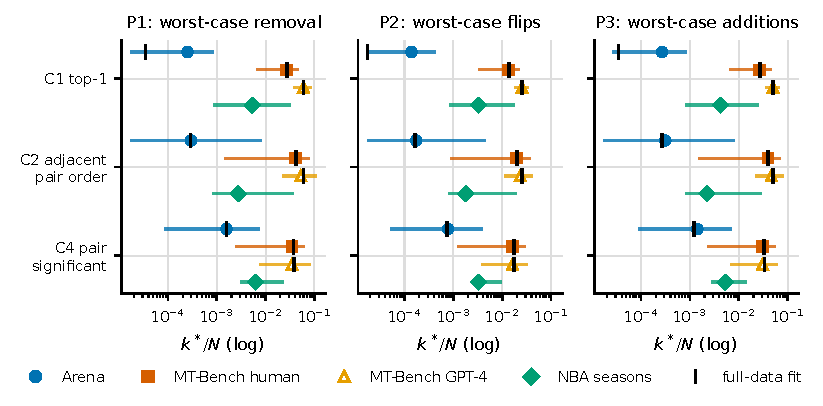
\includegraphics[width=\linewidth]{../figures/rendered/f1_fragility.pdf}
\caption{Worst-case edit size to change a ranking claim as a fraction of all comparisons ($\kst/N$, log scale), for removals (P1), label flips (P2) and added votes (P3) and claims C1, C2, C4. Dot: median; bar: 2.5--97.5 percentile over the replicate units of one dataset, pooled over claim instances; black tick: the single full-data fit. The bars show variation across replicates of a dataset, not a design-level confidence interval.}
\label{fig:frag}
\end{figure}

\subsection{Worst case versus random edits and sampling noise}
\label{sec:exp-base}
Where the claim is already within sampling noise, the worst case adds nothing beyond what noise does: the top-1 claim of Arena flips in \N{BFAC10} of full-size bootstrap resamples, and for NBA 2015 the order of the rank-3 and rank-4 teams in \N{BFNBC23}. Where the claim is well separated, resampling never moves it (MT-Bench human top-1 and Arena pair 2/3: \N{BFMHC10} and \N{BFAC22} of resamples) and random removals do not either: removing up to \N{RRMHkmax} judgments at random (\N{RRMHratio}$\times$ the worst-case $\kst$) never changed the MT-Bench-human top-1 in \N{RRnMH} draws; up to \N{RWAkmax} random battles ($\N{RWAratio}\times$ the worst case for the 2/3 pair) changed it in \N{RWAp} of \N{RWnA} draws. For the GPT-4-judge board the random baseline reaches only \N{RRMGkmax} removals (\N{RRMGratio}$\times$ $\kst$) and also never flips. The exception is the 2/3 pair of the human board (not significant: $z=\N{MHC2P12z}$, worst case $\kst=\N{MHC2P12k}$): \N{RWMHkmax} random removals (\N{RWMHratio}$\times$ the worst case) changed it in \N{RWMHp} of \N{RWnMH} draws. These ratios are lower bounds, because the random curves stop at the budget stated and show no flip there; the worst case is therefore at least this much smaller than a random loss of comparisons, and the gap between ``unlucky'' and ``adversarial'' grows with the separation of the claim (Figure~\ref{fig:random}).

\begin{figure}[t]
\centering
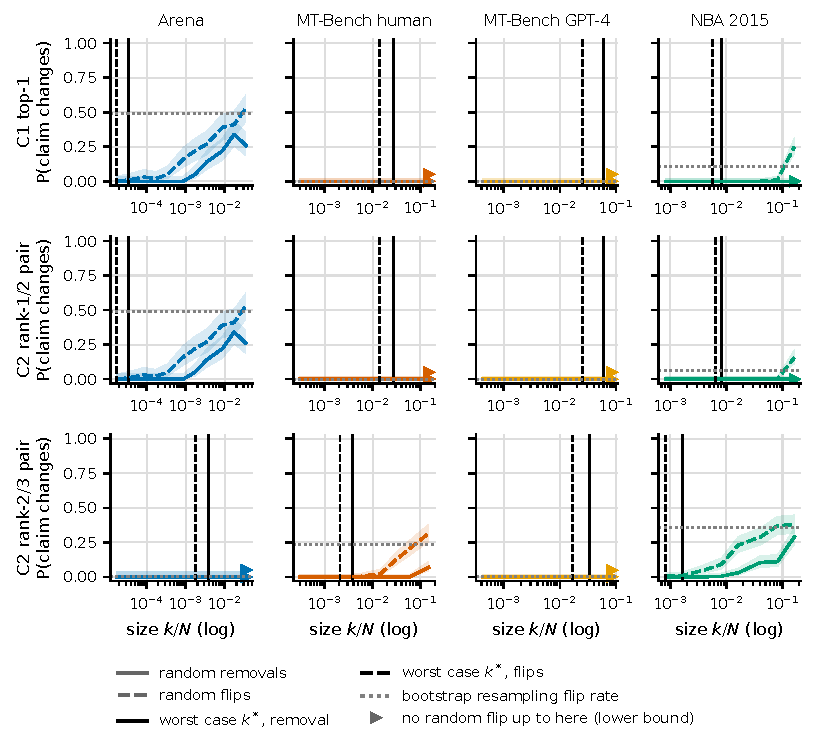
\includegraphics[width=\linewidth]{../figures/rendered/f2_worst_vs_random.pdf}
\caption{Random edits against the worst case. Curves: share of draws in which the claim fitted on the full data no longer holds after $k$ random removals (solid) or label flips (dashed), with 95\% Wilson bands (100--200 draws); vertical lines: worst-case $\kst$ for removals (solid) and flips (dashed); dotted horizontal line: share of bootstrap resamples of all comparisons in which the claim differs from the full-data fit. Rows: the top-1 claim (C1), the adjacent pair at ranks 1/2 and the pair at ranks 2/3 (C2). A right-pointing marker at the end of a curve means that no random edit changed the claim up to the largest size tried, so the ratio of that size to $\kst$ is a lower bound. The NBA panel is season 2015 only.}
\label{fig:random}
\end{figure}

\subsection{Do evaluation designs differ?}
\label{sec:exp-design}
\textbf{On the fraction $\kst/N$ they differ by two orders of magnitude} (Figure~\ref{fig:scales} in the appendix). The median over replicates of $\kst/N$ for an adjacent order claim (C2, removal) is \N{UNSC2P1kN} for NBA seasons, \N{UAC2P1kN} for Arena, \N{UMHC2P1kN} for MT-Bench expert and \N{UMGC2P1kN} for the GPT-4 judge. As a fraction of the comparisons that involve the two participants (s2) the spread is smaller: \N{UNSC2P1kNloc}, \N{UAC2P1kNloc}, \N{UMHC2P1kNloc}, \N{UMGC2P1kNloc}.

\textbf{The ordering follows how well separated the claims are} (Figure~\ref{fig:pred}). The median $z$ of these claims is \N{UNSC2P1z} (NBA), \N{UAC2P1z} (Arena), \N{UMHC2P1z} (MT-Bench human) and \N{UMGC2P1z} (GPT-4 judge), and the share of claims with $z<1.96$ (so not even significant in the data) is \N{UNSC2P1fz}, \N{UAC2P1fz}, \N{UMHC2P1fz} and \N{UMGC2P1fz}. Over all \N{SCC2rows} (dataset, replicate, claim) rows of the removal family, $\log\kst=c+\beta_z\log z+\beta_N\log N_{\mathrm{loc}}$ fits with $R^2=\N{SCC2r2}$ and residual s.d.\ \N{SCC2res} (log units), with $\beta_z=\N{SCC2uz}$ [\N{SCC2uzlo}, \N{SCC2uzhi}] and $\beta_N=\N{SCC2uN}$ [\N{SCC2uNlo}, \N{SCC2uNhi}] for C2 (similar for C1: $\beta_z=\N{SCC1uz}$, $R^2=\N{SCC1r2}$). The high $R^2$ is partly mechanical: $\kst$ is the number of edits needed to close a gap of $z$ standard errors, so it must grow with $z$ and with the local sample size. The fit describes how $\kst$ varies with claim separation; it does not explain why the separation differs between designs, which is where any design effect would sit. The pooled rows include the three LLM-judge boards on Arena battles (the \emph{model-judge} design together with the MT-Bench GPT-4 board). These intervals resample replicates within each dataset and the NBA seasons. Resampling datasets as clusters gives much wider ranges ($\beta_z\in$ [\N{SCC2dzlo}, \N{SCC2dzhi}], $\beta_N\in$ [\N{SCC2dNlo}, \N{SCC2dNhi}]), so the exponents are only loosely pinned down by the few independent datasets (NBA seasons, Arena with its judge relabellings, MT-Bench human, MT-Bench GPT-4); we read them as evidence that $\kst$ grows about linearly in the $z$-gap and sub-linearly in the local sample size, not as exact laws. For significance claims (C4), which are defined only above $z=1.96$, the slope is steeper ($\beta_z=\N{SCC4uz}$), as expected for a distance to a threshold. Adding design indicators changes the fit little ($R^2$ \N{SM0r2} to \N{SM1r2}) as a descriptive fit, not a causal explanation, and the dataset offsets are modest relative to the other variation: expert $\N{SMexpert}$, model judge (GPT-4 on MT-Bench and the Arena LLM judges) $\N{SMmodel}$, sports $\N{SMsports}$ log-units against crowd votes (factors \N{SFexpert}, \N{SFmodel}, \N{SFsports}; for adjacent-order removals, with no valid dataset-level interval since each design is a single dataset; across all \N{SDn} claim-by-perturbation fits the offsets range from \N{SDmin} to \N{SDmax} log-units, factors \N{SDfmin}--\N{SDfmax}, the sports offset being most negative for significance claims).

\textbf{Matched controls} (Figure~\ref{fig:size}). Size and sparsity alone do not make Arena fragile or robust: an Arena subset of the 6 best-covered models with the size of MT-Bench-human has a median C2 $\kst$ of \N{MAmtdenseC2med} (range \N{MAmtdenseC2lo}--\N{MAmtdenseC2hi}, \N{MAmtdenseC2kN} of $N$, median $z=\N{MAmtdenseC2z}$; \N{MAmtdenseC2n} draws), against \N{UMHC2P1med} for MT-Bench-human itself ($z=\N{UMHC2P1z}$); a 30-model sparse subset matched to an NBA season has a median of \N{MAnbalikeC2med} (\N{MAnbalikeC2lo}--\N{MAnbalikeC2hi}; $z=\N{MAnbalikeC2z}$; \N{MAnbalikeC2n} of 100 draws had all claims defined), like the NBA seasons (\N{UNSC2P1med}). The Arena models are closer in score than the MT-Bench ones, so their $z$ is lower at equal size, and $\kst$ follows $z$.

\textbf{Human versus GPT-4 judge on the same questions.} This is the cleanest design contrast (Figure~\ref{fig:matched}). On the same resampled questions, the GPT-4 board needs \N{PANC10}$\times$ as large a fraction of edits ($\kst/N$ ratio, median [95\% interval]) to change the top-1 claim, since its lead is larger (difference in $z$: \N{PAdzC10}); with one human judgment per aligned key the ratio is \N{PBNC10}. The same holds for the 2/3 pair (\N{PANC22}), but not for lower-ranked pairs, where the ratio is compatible with~1 (3/4 pair: \N{PANC23}). On MT-Bench the judge type therefore matters through how it spreads the models, not as a separate sensitivity. We cannot say how this generalises: there is one expert board and one GPT-4 judge.

\textbf{Crowd versus three LLM judges on identical Arena battles} (Figure~\ref{fig:judges} in the appendix). Here the top-1 claim is a near-tie on every board ($z=\N{JHC10z}$ for the human votes, \N{JLC10z}, \N{JTC10z}, \N{JQC10z} for the judges) and $\kst$ is small and not clearly different (human \N{JHC10k}; judges \N{JLC10k}, \N{JTC10k}, \N{JQC10k}; paired ratio judge/human \N{JRLC10}, \N{JRTC10}, \N{JRQC10}). For the pair at ranks 2/3 of each board, which is clearly significant everywhere ($z=\N{JHC22z}$ human; \N{JLC22z}, \N{JTC22z}, \N{JQC22z}), the judge boards need about a third of the removals ($\kst=\N{JHC22k}$ human vs.\ \N{JLC22k}, \N{JTC22k}, \N{JQC22k}; paired ratio \N{JRLC22}, \N{JRTC22}, \N{JRQC22}, 40 shared resamples) at nearly the same $z$. The pair may not consist of the same models on every board, and $z$ and $N_{\mathrm{loc}}$ do not capture this difference; Qwen's tie rate (\N{JQtie}) is close to the human one (\N{JHtie}) and its ratio is as low, which argues against the tie rate alone. The judges' tie rates differ from the human one (\N{JLtie}--\N{JQtie} against \N{JHtie}) and this is not separated from the other differences between the label sources. We did not identify the cause, so $z$ and local size are not the whole story for $\kst$ when the labels come from a different judge.

\begin{figure}[t]
\centering
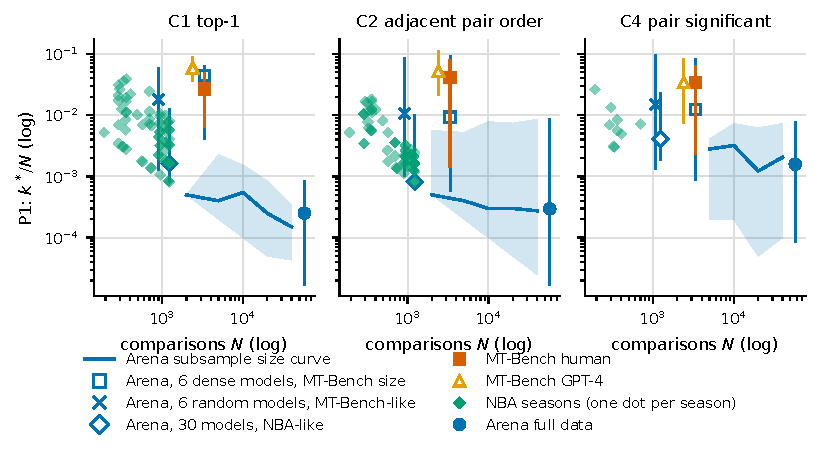
\includegraphics[width=\linewidth]{../figures/rendered/f4_size_control.pdf}
\caption{Size and sparsity control (s4), removal family. Arena subsampled to $N$ comparisons (line and band: median and 2.5--97.5 percentile over 30 draws), Arena subsets matched to MT-Bench (6 models, dense; 6 random models) and to an NBA season (30 models, sparse), against the real MT-Bench and NBA boards and the full Arena. A real board lying on the matched-Arena marker at the same $N$ is not distinguished from Arena by size and sparsity alone.}
\label{fig:size}
\end{figure}
\begin{figure}[t]
\centering
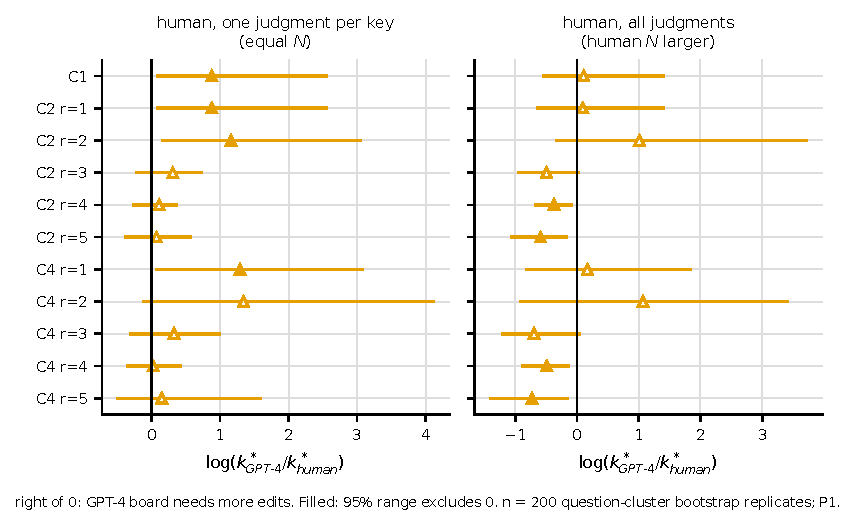
\includegraphics[width=\linewidth]{../figures/rendered/f5_matched_mtbench.pdf}
\caption{Matched human versus GPT-4 contrast, removal family: $\log(\kst_{\mathrm{GPT\text{-}4}}/\kst_{\mathrm{human}})$ on the same 200 question-cluster bootstrap replicates, per claim instance. Left: one random human judgment per (question, turn, model-pair) key, so equal $N$; right: all human judgments ($N$ about 1.85 times larger). Positive: the GPT-4 board needs more edits. Filled markers: the 95\% range excludes 0.}
\label{fig:matched}
\end{figure}
\begin{figure}[t]
\centering
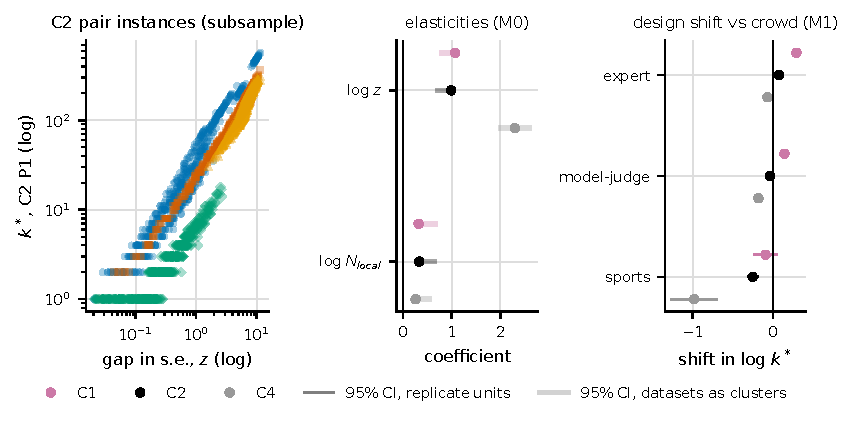
\includegraphics[width=\linewidth]{../figures/rendered/f6_predictors.pdf}
\caption{What predicts $\kst$ (removals). Left: $\kst$ against $z$ for C2 pair instances (800-point subsample per design, display only). Middle: log-log regression coefficients of $\kst$ on $z$ and $N_{\mathrm{loc}}$ (thin: bootstrap over replicate units, conditional on the datasets; wide pale: datasets as clusters, 12--72 clusters). Right: design shifts in $\log\kst$ relative to crowd votes (units bootstrap only). Descriptive, not a causal model.}
\label{fig:pred}
\end{figure}

\subsection{How loose is the search, and how robust are the results?}
\label{sec:exp-valid}
\textbf{The upper bound} (Figure~\ref{fig:valid} in the appendix). On \N{EXn} small instances (3-participant boards, exhaustive search up to $k=14$; \N{EXcap} of \N{EXall} instances were capped and are excluded), the greedy search with exact refit returned the exhaustive minimum in all \N{EXagree}. This certifies the search only on small boards: for the real boards $\kst$ remains an upper bound of unknown looseness. The influence prediction of the score-gap change is accurate for small edit budgets (median absolute relative error \N{APamed} at a quarter of $\kst$, \N{APbmed} at $\kst$ edits, worst case \N{APbmax} over \N{APn} cases) but a one-shot linear estimate of $\kst$ can be far off (GPT-4 judge top-1: \N{MGC1P10klin} predicted vs.\ \N{MGC1P10k} verified); we therefore always refit.

\textbf{Modelling choices} (Table~\ref{tab:sens}). Dropping ties (Arena 2/3 pair: $\kst$ \N{SEAtiehalf2} $\to$ \N{SEAtiedropped2}; MT-Bench human: \N{SEMHtiehalf2} $\to$ \N{SEMHtiedropped2}; GPT-4 judge \N{SEMGtiehalf2} $\to$ \N{SEMGtiedropped2}) changes $\kst$ by a factor up to about 2 and in either direction, and the Arena top-1 stays a near-tie ($\kst=\N{SEAtiedropped0}$). Without the home-advantage term the median NBA top-1 $\kst$ is \N{SENBnohome} (vs.\ \N{UNSC1P1med}), with playoffs \N{SENBwithplayoffs}. Pooling 5, 10, 20 seasons gives \N{SEnbapooled5}, \N{SEnbapooled10}, \N{SEnbapooled20} games for the top-1 claim. The ranker itself matters as much as an adversarial edit: online Elo with $K=4$ agrees with BT at Kendall $\tau=\N{ELA4tau}$ on Arena and $\N{ELA32tau}$ at $K=32$, and gives the same top-1 as the reference arrival order in only \N{ELA4top} of random orders ($K=4$). On NBA, BT agrees with FiveThirtyEight's Elo at $\tau=\N{SNtau}$ on average across \N{SNn} seasons (same top team in \N{SNsame}).

\textbf{Uncertainty scale.} The Wald standard error behind $z$ is within \N{SEratiomin}--\N{SEratiomax} of the bootstrap one (it is too large, hence $z$ conservative, by up to about 40\% on Arena and MT-Bench, where ties are treated as half-wins).



\section{Discussion and Limitations}
\label{sec:discussion}

\textbf{What the evidence supports.} For leaderboard claims between participants that the data cannot already separate (Arena top-1, the middle of an NBA season), changing a handful of comparisons is enough, but so is resampling: the worst-case size is not an extra vulnerability beyond what the published uncertainty already shows. For claims that are statistically significant, the number of comparisons needed is much larger than any random loss (random removals $\N{RRMHratio}\times$ as many never changed the MT-Bench-human top-1, and $\N{RWMHratio}\times$ as many changed its pair at ranks 2/3 in \N{RWMHp} of draws) yet remains small in relative terms: from about \N{UAC4P1kN} of the battles on Arena to a few percent on MT-Bench. A manipulator who needs $\kst$ edits may therefore succeed with a number of votes far below the sample size, in line with the vote-rigging concern~\cite{min2025rigging}, although our edits use full knowledge of the data and carry no cost or detectability constraint.

\textbf{Designs.} Differences in $\kst/N$ between crowd, expert, model-judge and sports data are large, but they are mostly accounted for by the separation of the claims and the local sample size; with those controlled the remaining dataset offsets are factors \N{SDfmin}--\N{SDfmax} in $\kst$ over all claims and perturbations (about 1.2 or less for adjacent-order removals); these are single-dataset contrasts, not estimated design effects. The matched human/GPT-4 contrast and the Arena subsets agree, but on identical Arena battles three LLM judges needed only about a third of the removals of the human votes to change a significant pair at nearly the same $z$, which the $z$-gap and local size do not explain. We do not claim a population-level design effect: each design is represented by a single dataset.

\textbf{Limitations.} (1)~$\kst$ is an upper bound found by greedy search with exact refits, certified against exhaustive search only on 3-participant boards. (2)~Four datasets (with three LLM-judge relabellings of one of them) and one ranking model: BT misspecification (intransitivity, judge position bias in the GPT-4 judge, non-stationarity of NBA and of Arena over time, user heterogeneity) is not modelled, and comparisons within a cell are treated as exchangeable although MT-Bench judgments share questions (handled in the intervals by the question-cluster bootstrap, not in the fit). (3)~Perturbations are mathematical edits to votes: additions are restricted to pairs containing the challenger; we make no claim about what a real manipulator can do or how detectable it is. (4)~The scaling fit is exploratory (fitted after seeing the results), its dataset-level uncertainty is wide, and replicates within a dataset are dependent. (5)~Not done: the larger Arena 140k set, and WebDev Arena were not analysed, and the LLM-judge labels on Arena battles (no declared licence, research use only) enter only the matched contrast above; there is no Arena time split (the 55k release has no timestamp or user column); the top-$k$ (C3) claim has no battle-bootstrap summary for Arena. (6)~The Arena top-1 is a statistical tie in this release, so fragility numbers for C1 on Arena say more about the tie than about the platform today.


\textbf{Broader impact.} Showing how few comparisons can change a ranking could help someone who wants to manipulate a leaderboard. We analyse existing public data only, release no attack tooling beyond the analysis code, and consider that operators benefit more from knowing which claims are close to a tie and which are not; we recommend reporting such margins next to rankings.

\section*{LLM assistance}
Large language models (Claude) were used throughout this study: for literature reading (abstract level), writing the analysis and plotting code, and drafting this text. The work was carried out by a set of automated agents with separate roles (analysis, figures, venue, writing, reviews). All numbers in this paper are produced by the committed code from the pinned public data and are read into the text by \texttt{paper/make\_numbers.py}; authors answer for the content. We did not open the starter-literature item on dropping preferences~\cite{huang2025dropping}, nor search for work citing it; no excluded material was encountered.

\bibliographystyle{plain}
{\small\bibliography{refs}}

\appendix
\section{Data, licences and reproduction}
\label{app:repro}
\begin{center}\small
\begin{tabular}{@{}p{0.46\linewidth}p{0.17\linewidth}p{0.11\linewidth}p{0.17\linewidth}@{}}
\toprule
Data & Version (commit) & Licence & Used\\\midrule
Chatbot Arena 55k votes (HF \texttt{lmarena-ai/arena-human-preference-55k}) & \texttt{18c29834\ldots} & apache-2.0 & yes\\
MT-Bench human/GPT-4 judgments (HF \texttt{lmsys/mt\_bench\_human\_judgments}) & \texttt{f7d2896d\ldots} & cc-by-4.0 & yes\\
NBA game records (FiveThirtyEight \texttt{nba-elo}) & \texttt{4c1ff5e3\ldots} & CC-BY-4.0 & yes\\
LLM-judge labels on Arena (HF \texttt{potsawee/chatbot-arena-llm-judges}) & \texttt{638a7e3b\ldots} & undeclared & yes, matched judge contrast only\\
\bottomrule
\end{tabular}
\end{center}
Full commits and sha256 checksums are in \texttt{code/README.md} and \texttt{results/MANIFEST.json}; raw data are not part of the delivery. Data are fetched and checked against pinned commits and sha256 values by \texttt{code/fetch\_data.sh}. Environment, seeds, run commands, expected run times (about one hour on two CPU cores for all analyses) and the script that produces each result file are in \texttt{code/README.md}; the figure and table generators are in \texttt{figures/}. \textbf{Excluded-source encounters:} none by any position (the starter-literature item on dropping preferences was not opened and no page citing it was read).

\paragraph{Script to figure and table map.} All figures and tables are produced by \path{figures/make_figures.py} from \path{results/} (input checksums in \path{figures/rendered/PROVENANCE.json}); numbers in the text are produced by \path{paper/make_numbers.py}. Table~\ref{tab:headline} and Figures~\ref{fig:frag}, \ref{fig:scales}: \path{kstar_full.csv}, \path{kstar_units.csv}; Figure~\ref{fig:random}: \path{random_curve.csv}, \path{boot_flip.csv}; Figure~\ref{fig:size}: \path{matched_arena.csv}; Figure~\ref{fig:matched}: \path{paired_mt.csv}; Figure~\ref{fig:pred}: \path{scaling_fit.csv}; Figure~\ref{fig:judges}: \path{kstar_judges.csv}, \path{paired_mt.csv}; Figure~\ref{fig:valid}: \path{exact_check.csv}, \path{approx_check.csv}; Tables~\ref{tab:data}, \ref{tab:sens}: \path{data_summary.csv}, \path{sensitivity.csv}.

\begin{figure}[h]
\centering
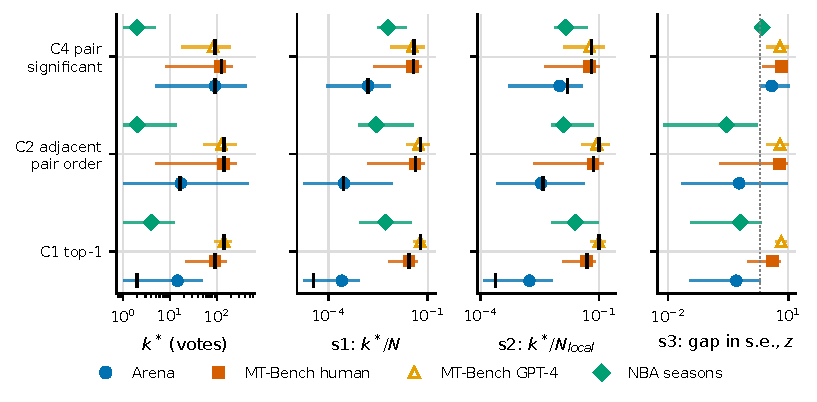
\includegraphics[width=\linewidth]{../figures/rendered/f3_scales.pdf}
\caption{The removal (P1) results of Figure~\ref{fig:frag} on four scales: absolute $\kst$, $\kst/N$ (s1), $\kst/N_{\mathrm{loc}}$ with $N_{\mathrm{loc}}$ the comparisons involving the claim's two participants (s2), and the claim's gap in standard errors $z$ (s3; dotted line: 1.96). Same bars as Figure~\ref{fig:frag}; the order of the designs changes with the scale.}
\label{fig:scales}
\end{figure}
\begin{figure}[h]
\centering
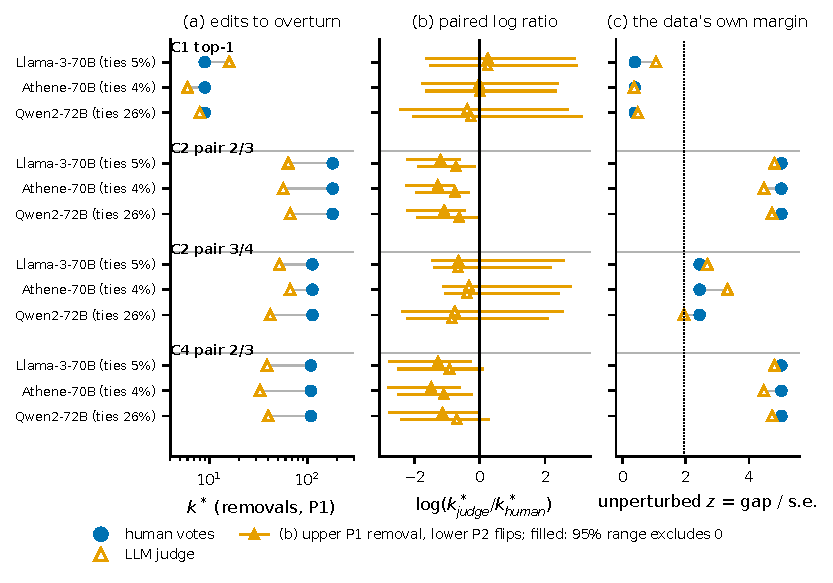
\includegraphics[width=\linewidth]{../figures/rendered/f8_crowd_vs_judges.pdf}
\caption{Crowd votes against three LLM judges on the same \N{JN} single-turn Arena battles (all boards refitted on them). Rows: C1 top-1, C2 order of the pairs at ranks 2/3 and 3/4, C4 significance of the 2/3 difference (ranks within each board's own ranking, so the pair need not be the same models). (a)~Full-data worst-case removals $\kst$, human (circle) and judge (triangle). (b)~Paired $\log(\kst_{\mathrm{judge}}/\kst_{\mathrm{human}})$ over 40 shared battle-bootstrap resamples, median and 2.5--97.5 percentile; upper bar removals, lower bar label flips; negative: the judge board needs fewer edits; filled: the range excludes 0. (c)~Unperturbed $z$ of the same pair (dotted: 1.96). Tie rates: human \N{JHtie}, judges \N{JLtie} (Llama), \N{JTtie} (Athene), \N{JQtie} (Qwen), so judge boards are not human boards with a different scorer; the resamples give only a within-dataset range, not a design-level interval.}
\label{fig:judges}
\end{figure}
\begin{figure}[h]
\centering
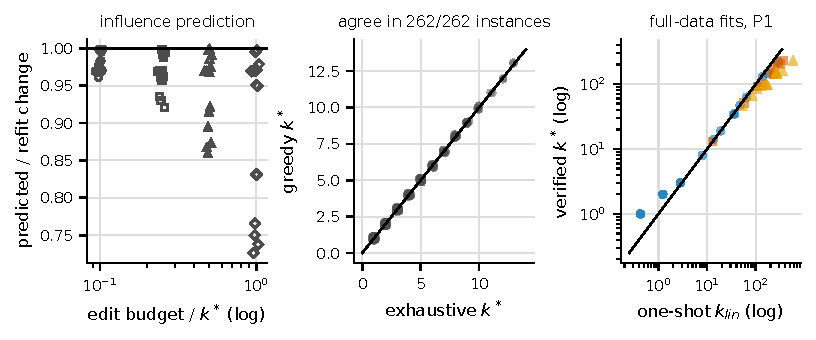
\includegraphics[width=\linewidth]{../figures/rendered/f7_search_validity.pdf}
\caption{Validity of the search (removals). Left: influence-predicted over exactly refitted change of the claim margin for edit budgets of 10--100\% of $\kst$. Middle: greedy against exhaustive $\kst$ on small instances (capped searches excluded); the title gives the agreement count. Right: one-shot linear prediction against the verified $\kst$ on the full-data fits.}
\label{fig:valid}
\end{figure}
\begin{table}[h]
\centering
\caption{The boards: comparisons $N$, participants, comparisons per participant, tie rate and standard deviation of the BT scores (log scale). Source: \texttt{results/data\_summary.csv}.}
\label{tab:data}
{\footnotesize\setlength{\tabcolsep}{3pt}
\begin{tabular}{llrrrrr}
\toprule
Board & Design & $N$ & Participants & Cmp./participant & Tie rate & Score s.d. \\
\midrule
nba\_2015 & sports & 1230 & 30 & 82 & 0.00 & 0.80 \\
mtbench\_human & expert & 3355 & 6 & 1118 & 0.23 & 0.86 \\
mtbench\_gpt4 & model-judge & 2400 & 6 & 800 & 0.25 & 1.28 \\
arena55k & crowd & 57477 & 64 & 1796 & 0.31 & 0.56 \\
nba\_1950 & sports & 561 & 17 & 66 & 0.00 & 0.95 \\
nba\_1970 & sports & 574 & 14 & 82 & 0.00 & 0.47 \\
nba\_1990 & sports & 1107 & 27 & 82 & 0.00 & 0.91 \\
nba\_2005 & sports & 1230 & 30 & 82 & 0.00 & 0.75 \\
nba\_2010 & sports & 1230 & 30 & 82 & 0.00 & 0.80 \\
\bottomrule
\end{tabular}
}

\end{table}
\begin{table}[h]
\centering
\caption{Ratio of $\kst$ under a modelling variant to the reference fit for the same claim instance (median; IQR over instances); pooled NBA windows are different boards and are reported as $\kst/N$. Source: \texttt{results/sensitivity.csv}.}
\label{tab:sens}
{\footnotesize\setlength{\tabcolsep}{3pt}
\begin{tabular}{llllr}
\toprule
Board & Variant & Claim & Median ratio $k^*_{var}/k^*_{ref}$ [IQR] & $n$ \\
\midrule
arena55k & tie\_dropped & C1 & 4.50 [4.50, 4.50] & 1 \\
arena55k & tie\_dropped & C2 & 0.97 [0.79, 1.73] & 10 \\
arena55k & tie\_dropped & C4 & 1.79 [1.56, 2.03] & 2 \\
mtbench\_human & tie\_dropped & C1 & 0.90 [0.90, 0.90] & 1 \\
mtbench\_human & tie\_dropped & C2 & 0.81 [0.79, 0.86] & 5 \\
mtbench\_human & tie\_dropped & C4 & 0.88 [0.86, 0.92] & 4 \\
mtbench\_gpt4 & tie\_dropped & C1 & 0.52 [0.52, 0.52] & 1 \\
mtbench\_gpt4 & tie\_dropped & C2 & 0.56 [0.54, 0.89] & 5 \\
mtbench\_gpt4 & tie\_dropped & C4 & 0.71 [0.65, 1.08] & 5 \\
nba\_season & no\_home & C1 & 1.00 [1.00, 1.25] & 69 \\
nba\_season & no\_home & C2 & 1.00 [1.00, 1.03] & 631 \\
nba\_season & no\_home & C4 & 1.40 [1.00, 1.50] & 7 \\
nba\_season & with\_playoffs & C1 & 1.00 [0.80, 1.60] & 69 \\
nba\_season & with\_playoffs & C2 & 1.00 [0.75, 1.50] & 650 \\
nba\_season & with\_playoffs & C4 & 1.00 [1.00, 1.00] & 7 \\
nba\_pooled & pooled\_10 & C1 & median $k^*/N$ = 0.0048 & 1 \\
nba\_pooled & pooled\_10 & C2 & median $k^*/N$ = 0.001 & 10 \\
nba\_pooled & pooled\_20 & C1 & median $k^*/N$ = 0.002 & 1 \\
nba\_pooled & pooled\_20 & C2 & median $k^*/N$ = 0.00036 & 10 \\
nba\_pooled & pooled\_5 & C1 & median $k^*/N$ = 0.0039 & 1 \\
nba\_pooled & pooled\_5 & C2 & median $k^*/N$ = 0.0011 & 10 \\
\bottomrule
\end{tabular}
}

\end{table}

\section*{NeurIPS Paper Checklist}




\begin{enumerate}

\item {\bf Claims}
    \item[] Question: Do the main claims made in the abstract and introduction accurately reflect the paper's contributions and scope?
    \item[] Answer: \answerYes{}
    \item[] Justification: Abstract and introduction state the claims, their conditions and the limits; Sections~\ref{sec:experiments} and~\ref{sec:discussion} support them.
    \item[] Guidelines:
    \begin{itemize}
        \item The answer \answerNA{} means that the abstract and introduction do not include the claims made in the paper.
        \item The abstract and/or introduction should clearly state the claims made, including the contributions made in the paper and important assumptions and limitations. A \answerNo{} or \answerNA{} answer to this question will not be perceived well by the reviewers. 
        \item The claims made should match theoretical and experimental results, and reflect how much the results can be expected to generalize to other settings. 
        \item It is fine to include aspirational goals as motivation as long as it is clear that these goals are not attained by the paper. 
    \end{itemize}

\item {\bf Limitations}
    \item[] Question: Does the paper discuss the limitations of the work performed by the authors?
    \item[] Answer: \answerYes{}
    \item[] Justification: Section~\ref{sec:discussion} (Limitations) lists the upper-bound nature of $\kst$, four datasets, BT misspecification, restricted additions and work not done.
    \item[] Guidelines:
    \begin{itemize}
        \item The answer \answerNA{} means that the paper has no limitation while the answer \answerNo{} means that the paper has limitations, but those are not discussed in the paper. 
        \item The authors are encouraged to create a separate ``Limitations'' section in their paper.
        \item The paper should point out any strong assumptions and how robust the results are to violations of these assumptions (e.g., independence assumptions, noiseless settings, model well-specification, asymptotic approximations only holding locally). The authors should reflect on how these assumptions might be violated in practice and what the implications would be.
        \item The authors should reflect on the scope of the claims made, e.g., if the approach was only tested on a few datasets or with a few runs. In general, empirical results often depend on implicit assumptions, which should be articulated.
        \item The authors should reflect on the factors that influence the performance of the approach. For example, a facial recognition algorithm may perform poorly when image resolution is low or images are taken in low lighting. Or a speech-to-text system might not be used reliably to provide closed captions for online lectures because it fails to handle technical jargon.
        \item The authors should discuss the computational efficiency of the proposed algorithms and how they scale with dataset size.
        \item If applicable, the authors should discuss possible limitations of their approach to address problems of privacy and fairness.
        \item While the authors might fear that complete honesty about limitations might be used by reviewers as grounds for rejection, a worse outcome might be that reviewers discover limitations that aren't acknowledged in the paper. The authors should use their best judgment and recognize that individual actions in favor of transparency play an important role in developing norms that preserve the integrity of the community. Reviewers will be specifically instructed to not penalize honesty concerning limitations.
    \end{itemize}

\item {\bf Theory assumptions and proofs}
    \item[] Question: For each theoretical result, does the paper provide the full set of assumptions and a complete (and correct) proof?
    \item[] Answer: \answerNA{}
    \item[] Justification: The paper states no theorem; the influence approximation is used as a heuristic and every result is verified by exact refitting.
    \item[] Guidelines:
    \begin{itemize}
        \item The answer \answerNA{} means that the paper does not include theoretical results. 
        \item All the theorems, formulas, and proofs in the paper should be numbered and cross-referenced.
        \item All assumptions should be clearly stated or referenced in the statement of any theorems.
        \item The proofs can either appear in the main paper or the supplemental material, but if they appear in the supplemental material, the authors are encouraged to provide a short proof sketch to provide intuition. 
        \item Inversely, any informal proof provided in the core of the paper should be complemented by formal proofs provided in appendix or supplemental material.
        \item Theorems and Lemmas that the proof relies upon should be properly referenced. 
    \end{itemize}

    \item {\bf Experimental result reproducibility}
    \item[] Question: Does the paper fully disclose all the information needed to reproduce the main experimental results of the paper to the extent that it affects the main claims and/or conclusions of the paper (regardless of whether the code and data are provided or not)?
    \item[] Answer: \answerYes{}
    \item[] Justification: Sections~\ref{sec:method} and~\ref{sec:experiments} and Appendix~\ref{app:repro} give data versions, fitting, search and replication; \texttt{code/README.md} lists commands, seeds and the script behind each result file.
    \item[] Guidelines:
    \begin{itemize}
        \item The answer \answerNA{} means that the paper does not include experiments.
        \item If the paper includes experiments, a \answerNo{} answer to this question will not be perceived well by the reviewers: Making the paper reproducible is important, regardless of whether the code and data are provided or not.
        \item If the contribution is a dataset and\slash or model, the authors should describe the steps taken to make their results reproducible or verifiable. 
        \item Depending on the contribution, reproducibility can be accomplished in various ways. For example, if the contribution is a novel architecture, describing the architecture fully might suffice, or if the contribution is a specific model and empirical evaluation, it may be necessary to either make it possible for others to replicate the model with the same dataset, or provide access to the model. In general. releasing code and data is often one good way to accomplish this, but reproducibility can also be provided via detailed instructions for how to replicate the results, access to a hosted model (e.g., in the case of a large language model), releasing of a model checkpoint, or other means that are appropriate to the research performed.
        \item While NeurIPS does not require releasing code, the conference does require all submissions to provide some reasonable avenue for reproducibility, which may depend on the nature of the contribution. For example
        \begin{enumerate}
            \item If the contribution is primarily a new algorithm, the paper should make it clear how to reproduce that algorithm.
            \item If the contribution is primarily a new model architecture, the paper should describe the architecture clearly and fully.
            \item If the contribution is a new model (e.g., a large language model), then there should either be a way to access this model for reproducing the results or a way to reproduce the model (e.g., with an open-source dataset or instructions for how to construct the dataset).
            \item We recognize that reproducibility may be tricky in some cases, in which case authors are welcome to describe the particular way they provide for reproducibility. In the case of closed-source models, it may be that access to the model is limited in some way (e.g., to registered users), but it should be possible for other researchers to have some path to reproducing or verifying the results.
        \end{enumerate}
    \end{itemize}


\item {\bf Open access to data and code}
    \item[] Question: Does the paper provide open access to the data and code, with sufficient instructions to faithfully reproduce the main experimental results, as described in supplemental material?
    \item[] Answer: \answerYes{}
    \item[] Justification: All data are public with pinned versions and checksums (Appendix~\ref{app:repro}); the code and per-script reproduction steps are in the delivery (\texttt{code/README.md}); raw data are not redistributed.
    \item[] Guidelines:
    \begin{itemize}
        \item The answer \answerNA{} means that paper does not include experiments requiring code.
        \item Please see the NeurIPS code and data submission guidelines (\url{https://neurips.cc/public/guides/CodeSubmissionPolicy}) for more details.
        \item While we encourage the release of code and data, we understand that this might not be possible, so \answerNo{} is an acceptable answer. Papers cannot be rejected simply for not including code, unless this is central to the contribution (e.g., for a new open-source benchmark).
        \item The instructions should contain the exact command and environment needed to run to reproduce the results. See the NeurIPS code and data submission guidelines (\url{https://neurips.cc/public/guides/CodeSubmissionPolicy}) for more details.
        \item The authors should provide instructions on data access and preparation, including how to access the raw data, preprocessed data, intermediate data, and generated data, etc.
        \item The authors should provide scripts to reproduce all experimental results for the new proposed method and baselines. If only a subset of experiments are reproducible, they should state which ones are omitted from the script and why.
        \item At submission time, to preserve anonymity, the authors should release anonymized versions (if applicable).
        \item Providing as much information as possible in supplemental material (appended to the paper) is recommended, but including URLs to data and code is permitted.
    \end{itemize}


\item {\bf Experimental setting/details}
    \item[] Question: Does the paper specify all the training and test details (e.g., data splits, hyperparameters, how they were chosen, type of optimizer) necessary to understand the results?
    \item[] Answer: \answerYes{}
    \item[] Justification: Sections~\ref{sec:method} and~\ref{sec:experiments} define models, tie handling, perturbations, search and replication units; seeds and settings are in \texttt{code/README.md} and \texttt{results/MANIFEST.json}.
    \item[] Guidelines:
    \begin{itemize}
        \item The answer \answerNA{} means that the paper does not include experiments.
        \item The experimental setting should be presented in the core of the paper to a level of detail that is necessary to appreciate the results and make sense of them.
        \item The full details can be provided either with the code, in appendix, or as supplemental material.
    \end{itemize}

\item {\bf Experiment statistical significance}
    \item[] Question: Does the paper report error bars suitably and correctly defined or other appropriate information about the statistical significance of the experiments?
    \item[] Answer: \answerYes{}
    \item[] Justification: Replicate ranges and bootstrap intervals are reported (Section~\ref{sec:experiments}); the replication unit differs by dataset and is stated, and intervals that resample whole datasets are given where only four designs exist.
    \item[] Guidelines:
    \begin{itemize}
        \item The answer \answerNA{} means that the paper does not include experiments.
        \item The authors should answer \answerYes{} if the results are accompanied by error bars, confidence intervals, or statistical significance tests, at least for the experiments that support the main claims of the paper.
        \item The factors of variability that the error bars are capturing should be clearly stated (for example, train/test split, initialization, random drawing of some parameter, or overall run with given experimental conditions).
        \item The method for calculating the error bars should be explained (closed form formula, call to a library function, bootstrap, etc.)
        \item The assumptions made should be given (e.g., Normally distributed errors).
        \item It should be clear whether the error bar is the standard deviation or the standard error of the mean.
        \item It is OK to report 1-sigma error bars, but one should state it. The authors should preferably report a 2-sigma error bar than state that they have a 96\% CI, if the hypothesis of Normality of errors is not verified.
        \item For asymmetric distributions, the authors should be careful not to show in tables or figures symmetric error bars that would yield results that are out of range (e.g., negative error rates).
        \item If error bars are reported in tables or plots, the authors should explain in the text how they were calculated and reference the corresponding figures or tables in the text.
    \end{itemize}

\item {\bf Experiments compute resources}
    \item[] Question: For each experiment, does the paper provide sufficient information on the computer resources (type of compute workers, memory, time of execution) needed to reproduce the experiments?
    \item[] Answer: \answerYes{}
    \item[] Justification: CPU only; the full analysis takes about one hour on two CPU cores, per-script times in \texttt{code/README.md} (Appendix~\ref{app:repro}).
    \item[] Guidelines:
    \begin{itemize}
        \item The answer \answerNA{} means that the paper does not include experiments.
        \item The paper should indicate the type of compute workers CPU or GPU, internal cluster, or cloud provider, including relevant memory and storage.
        \item The paper should provide the amount of compute required for each of the individual experimental runs as well as estimate the total compute. 
        \item The paper should disclose whether the full research project required more compute than the experiments reported in the paper (e.g., preliminary or failed experiments that didn't make it into the paper). 
    \end{itemize}
    
\item {\bf Code of ethics}
    \item[] Question: Does the research conducted in the paper conform, in every respect, with the NeurIPS Code of Ethics \url{https://neurips.cc/public/EthicsGuidelines}?
    \item[] Answer: \answerYes{}
    \item[] Justification: The study re-analyses public data and follows the NeurIPS Code of Ethics; no deviation was identified.
    \item[] Guidelines:
    \begin{itemize}
        \item The answer \answerNA{} means that the authors have not reviewed the NeurIPS Code of Ethics.
        \item If the authors answer \answerNo, they should explain the special circumstances that require a deviation from the Code of Ethics.
        \item The authors should make sure to preserve anonymity (e.g., if there is a special consideration due to laws or regulations in their jurisdiction).
    \end{itemize}


\item {\bf Broader impacts}
    \item[] Question: Does the paper discuss both potential positive societal impacts and negative societal impacts of the work performed?
    \item[] Answer: \answerYes{}
    \item[] Justification: Broader impact in Section~\ref{sec:discussion}: sensitivity findings could inform manipulation as well as defence; no attack tooling beyond the analysis is released.
    \item[] Guidelines:
    \begin{itemize}
        \item The answer \answerNA{} means that there is no societal impact of the work performed.
        \item If the authors answer \answerNA{} or \answerNo, they should explain why their work has no societal impact or why the paper does not address societal impact.
        \item Examples of negative societal impacts include potential malicious or unintended uses (e.g., disinformation, generating fake profiles, surveillance), fairness considerations (e.g., deployment of technologies that could make decisions that unfairly impact specific groups), privacy considerations, and security considerations.
        \item The conference expects that many papers will be foundational research and not tied to particular applications, let alone deployments. However, if there is a direct path to any negative applications, the authors should point it out. For example, it is legitimate to point out that an improvement in the quality of generative models could be used to generate Deepfakes for disinformation. On the other hand, it is not needed to point out that a generic algorithm for optimizing neural networks could enable people to train models that generate Deepfakes faster.
        \item The authors should consider possible harms that could arise when the technology is being used as intended and functioning correctly, harms that could arise when the technology is being used as intended but gives incorrect results, and harms following from (intentional or unintentional) misuse of the technology.
        \item If there are negative societal impacts, the authors could also discuss possible mitigation strategies (e.g., gated release of models, providing defenses in addition to attacks, mechanisms for monitoring misuse, mechanisms to monitor how a system learns from feedback over time, improving the efficiency and accessibility of ML).
    \end{itemize}
    
\item {\bf Safeguards}
    \item[] Question: Does the paper describe safeguards that have been put in place for responsible release of data or models that have a high risk for misuse (e.g., pre-trained language models, image generators, or scraped datasets)?
    \item[] Answer: \answerNA{}
    \item[] Justification: No new dataset or model is released; the Arena text is not redistributed.
    \item[] Guidelines:
    \begin{itemize}
        \item The answer \answerNA{} means that the paper poses no such risks.
        \item Released models that have a high risk for misuse or dual-use should be released with necessary safeguards to allow for controlled use of the model, for example by requiring that users adhere to usage guidelines or restrictions to access the model or implementing safety filters. 
        \item Datasets that have been scraped from the Internet could pose safety risks. The authors should describe how they avoided releasing unsafe images.
        \item We recognize that providing effective safeguards is challenging, and many papers do not require this, but we encourage authors to take this into account and make a best faith effort.
    \end{itemize}

\item {\bf Licenses for existing assets}
    \item[] Question: Are the creators or original owners of assets (e.g., code, data, models), used in the paper, properly credited and are the license and terms of use explicitly mentioned and properly respected?
    \item[] Answer: \answerYes{}
    \item[] Justification: Data licences and versions are listed in Appendix~\ref{app:repro} (Arena 55k apache-2.0, MT-Bench cc-by-4.0, NBA CC-BY-4.0); the LLM-judge verdict set has no declared licence; it is used for research analysis only, in one matched contrast, and its raw files are not redistributed.
    \item[] Guidelines:
    \begin{itemize}
        \item The answer \answerNA{} means that the paper does not use existing assets.
        \item The authors should cite the original paper that produced the code package or dataset.
        \item The authors should state which version of the asset is used and, if possible, include a URL.
        \item The name of the license (e.g., CC-BY 4.0) should be included for each asset.
        \item For scraped data from a particular source (e.g., website), the copyright and terms of service of that source should be provided.
        \item If assets are released, the license, copyright information, and terms of use in the package should be provided. For popular datasets, \url{paperswithcode.com/datasets} has curated licenses for some datasets. Their licensing guide can help determine the license of a dataset.
        \item For existing datasets that are re-packaged, both the original license and the license of the derived asset (if it has changed) should be provided.
        \item If this information is not available online, the authors are encouraged to reach out to the asset's creators.
    \end{itemize}

\item {\bf New assets}
    \item[] Question: Are new assets introduced in the paper well documented and is the documentation provided alongside the assets?
    \item[] Answer: \answerYes{}
    \item[] Justification: The only new asset is the analysis code, documented in \texttt{code/README.md}.
    \item[] Guidelines:
    \begin{itemize}
        \item The answer \answerNA{} means that the paper does not release new assets.
        \item Researchers should communicate the details of the dataset\slash code\slash model as part of their submissions via structured templates. This includes details about training, license, limitations, etc. 
        \item The paper should discuss whether and how consent was obtained from people whose asset is used.
        \item At submission time, remember to anonymize your assets (if applicable). You can either create an anonymized URL or include an anonymized zip file.
    \end{itemize}

\item {\bf Crowdsourcing and research with human subjects}
    \item[] Question: For crowdsourcing experiments and research with human subjects, does the paper include the full text of instructions given to participants and screenshots, if applicable, as well as details about compensation (if any)? 
    \item[] Answer: \answerNA{}
    \item[] Justification: Secondary analysis of existing public data; no crowdsourcing or human subjects work by the authors.
    \item[] Guidelines:
    \begin{itemize}
        \item The answer \answerNA{} means that the paper does not involve crowdsourcing nor research with human subjects.
        \item Including this information in the supplemental material is fine, but if the main contribution of the paper involves human subjects, then as much detail as possible should be included in the main paper. 
        \item According to the NeurIPS Code of Ethics, workers involved in data collection, curation, or other labor should be paid at least the minimum wage in the country of the data collector. 
    \end{itemize}

\item {\bf Institutional review board (IRB) approvals or equivalent for research with human subjects}
    \item[] Question: Does the paper describe potential risks incurred by study participants, whether such risks were disclosed to the subjects, and whether Institutional Review Board (IRB) approvals (or an equivalent approval/review based on the requirements of your country or institution) were obtained?
    \item[] Answer: \answerNA{}
    \item[] Justification: No human-subjects research was conducted by the authors.
    \item[] Guidelines:
    \begin{itemize}
        \item The answer \answerNA{} means that the paper does not involve crowdsourcing nor research with human subjects.
        \item Depending on the country in which research is conducted, IRB approval (or equivalent) may be required for any human subjects research. If you obtained IRB approval, you should clearly state this in the paper. 
        \item We recognize that the procedures for this may vary significantly between institutions and locations, and we expect authors to adhere to the NeurIPS Code of Ethics and the guidelines for their institution. 
        \item For initial submissions, do not include any information that would break anonymity (if applicable), such as the institution conducting the review.
    \end{itemize}

\item {\bf Declaration of LLM usage}
    \item[] Question: Does the paper describe the usage of LLMs if it is an important, original, or non-standard component of the core methods in this research? Note that if the LLM is used only for writing, editing, or formatting purposes and does \emph{not} impact the core methodology, scientific rigor, or originality of the research, declaration is not required.
    %this research? 
    \item[] Answer: \answerYes{}
    \item[] Justification: LLM assistance in reading, coding and writing is declared in the section ``LLM assistance''; no LLM is a component of the method.
    \item[] Guidelines:
    \begin{itemize}
        \item The answer \answerNA{} means that the core method development in this research does not involve LLMs as any important, original, or non-standard components.
        \item Please refer to our LLM policy in the NeurIPS handbook for what should or should not be described.
    \end{itemize}

\end{enumerate}
\end{document}
